\documentclass[a4paper,oneside,12pt]{book}

%----------------------------------------------------------------------------------------
%	README!
%   Welcome. It's worth having a read through this file
%   to set up the broad parameters, such as the name of
%   the degree, the school/department, the type of work
%   (dissertation/Final Year Project/report, etc. as well
%   as your details.
%----------------------------------------------------------------------------------------

%----------------------------------------------------------------------------------------
%	COVER PAGE
%   The cover page is laid out in title/title.tex. You can choose a color
%   or black and white logo
%----------------------------------------------------------------------------------------

%----------------------------------------------------------------------------------------
%	THESIS INFORMATION
%   Put title, author name, supervisor name, degree, type of work, school, department in here
%   It will be used for the title page and the embedded PDF information
%----------------------------------------------------------------------------------------

\newcommand{\thesistitle}{MERIT.jl: Julia's Version} % Your thesis title, this is used in the title and abstract
\newcommand{\degree}{MAI (Electronic and Computer Engineering)} % Replace with your degree name, this is used in the title page and abstract
\newcommand{\typeofthesis}{Final Year Project} % dissertation, Final Year Project, report, etc.
\newcommand{\authorname}{Aaron Dinesh} % Your name, this is used in the title page and PDF stuff
%% Do not put your Student ID in the document, as TCD will not publish
%% documents that contain both your name and your Student ID.
\newcommand{\supervisor}{Dr. Declan O'Loughlin} % replace with the name of your supervisor
%\newcommand{\cosupervisor}{Dr. Alex Lee} % replace with the name of your co-supervisor if you have one
\newcommand{\keywords}{Microwave Imaging, Breast Imaging, Julia} % Replace with keywords for your thesis
\newcommand{\school}{\href{https://www.tcd.ie/Engineering/}{School of Engineering}} % Your school's name and URL, this is used in the title page
%Edited by HS for engineering

%% Comment out the next line if you don't want a department to appear
\newcommand{\department}{\href{https://www.tcd.ie/eleceng/}{Electronic and Electrical Engineering}} % Your research group's name and URL, this is used in the title page


%% Language and font encodings
\usepackage[T1]{fontenc} 
\usepackage[utf8]{inputenc}
\usepackage[english]{babel}
\usepackage{ulem}
%% Bibliographical stuff
\usepackage[]{cite}
%% Document size
%Include showframe as an option if you want to see the boxes
\usepackage[a4paper,top=2.54cm,bottom=2.54cm,left=2.54cm, right=2.54cm,headheight=16pt]{geometry}
\setlength{\marginparwidth}{2cm}
%% Useful packages
\usepackage{amsmath}
\usepackage[autostyle=true]{csquotes} % Required to generate language-dependent quotes in the bibliography
\usepackage[pdftex]{graphicx}
\usepackage[colorinlistoftodos]{todonotes}
\usepackage[colorlinks=true, allcolors=black]{hyperref}
\usepackage{hyperxmp}
\usepackage{caption} % if no caption, no colon
\usepackage{sfmath} %use sans-serif in the maths sections too
\usepackage[parfill]{parskip}    % Begin paragraphs with an empty line rather than an indent
\usepackage{setspace} % to permit one-and-a-half or double spacing
\usepackage{enumerate} % fancy enumerations like (i) (ii) or (a) (b) and such
\usepackage{booktabs} % To thicken table lines
\usepackage{fancyhdr}
\usepackage{xcolor} % to get TCD color on headings
\usepackage{hvfloat}
\usepackage{listings}
\usepackage{subcaption}
\usepackage{placeins}
\usepackage{xargs}                      % Use more than one optional parameter in a new commands
\captionsetup[figure]{font={default, sf}}
\setcounter{tocdepth}{4}
\graphicspath{{./Images/}}
\numberwithin{equation}{chapter} %HS edit for (chapter.equation)
\pagestyle{plain} % Embrace simplicity!
\counterwithout{figure}{section}
\definecolor{tcd_blue}{RGB}{5, 105, 185}
\newcommandx{\change}[2][1=]{\todo[linecolor=blue,backgroundcolor=blue!25,bordercolor=blue,#1]{#2}}

%% For Today's Date
\renewcommand{\today}{\ifnum\number\day<10 0\fi \number\day \space%
\ifcase \month \or January\or February\or March\or April\or May%
\or June\or July\or August\or September\or October\or November\or December\fi \space%
\number \year}

%% Defining Code Colors
\definecolor{codegreen}{rgb}{0,0.6,0}
\definecolor{codegray}{rgb}{0.5,0.5,0.5}
\definecolor{codepurple}{rgb}{0.58,0,0.82}
\definecolor{backcolour}{rgb}{0.95,0.95,0.92}

\lstdefinestyle{codeStyle}{
    backgroundcolor=\color{backcolour},   
    commentstyle=\color{codegreen},
    keywordstyle=\color{magenta},
    numberstyle=\tiny\color{codegray},
    stringstyle=\color{codepurple},
    basicstyle=\ttfamily\footnotesize,
    breakatwhitespace=false,         
    breaklines=true,                 
    captionpos=b,                    
    keepspaces=true,                 
    numbers=left,                    
    numbersep=5pt,                  
    showspaces=false,                
    showstringspaces=false,
    showtabs=false,                  
    tabsize=2
}

\lstset{style=codeStyle}

\lstdefinelanguage{Julia}%
  {morekeywords={abstract,break,case,catch,const,continue,do,else,elseif,%
      end,export,false,for,function,immutable,import,importall,if,in,%
      macro,module,otherwise,quote,return,switch,true,try,type,typealias,%
      using,while,struct,mutable},%
   sensitive=true,%
   alsoother={\$},%
   morecomment=[l]\#,%
   morecomment=[n]{\#=}{=\#},%
   morestring=[s]{"}{"},%
   morestring=[m]{'}{'},%
}[keywords,comments,strings]%

\lstset{%
    language         = Julia,
    basicstyle       = \ttfamily,
    keywordstyle     = \bfseries\color{magenta},
    stringstyle      = \color{codepurple},
    commentstyle     = \color{codegreen},
    showstringspaces = false,
}



%% It's personal taste but...
%% Uncomment the following block if you want your name and ID at the top of
%% (almost) every page.

%\pagestyle{fancy}
%\fancyhf{} % sets both header and footer to nothing
%\renewcommand{\headrulewidth}{0pt}
%\cfoot{\thepage}
%\ifdefined\authorid
%\chead{\it \authorname\ (\authorid)}
%\else
%\chead{\it \authorname}
%\fi
%% End of block

%% It is good practice to make your font sans-serif to improve the accessibility of your document.  Comment out the following line to disable it (but you really should not)
\renewcommand{\familydefault}{\sfdefault} %use the sans-serif font as default

%% If you insist on not using sans-serif (please don't), consider using Palatino instead of the LaTeX standard
%\usepackage{mathpazo} % Use the Palatino font by default if you prefer it to Computer Modern


%% Format Chapter headings appropriately
\usepackage{titlesec}
\titleformat{\chapter}[hang]{\normalfont\huge\bfseries\color{tcd_blue}}{\thechapter}{1cm}{}{}

\title{\thesistitle}
\author{\authorname}

\hypersetup{
   pdftitle=\thesistitle, % Set the PDF's title to your title
   pdfauthor=\authorname, % Set the PDF's author to your name
   pdfkeywords=\keywords, % Set the PDF's keywords to your keywords
   pdfsubject=\degree, % Set the PDF's keywords to your keywords
   pdfinfo={
     pdfsupervisor=\supervisor, % Set the PDF's supervisor to your supervisor
     %pdfcosupervisor=\cosupervisor, % Set the PDF's cosupervisor to your cosupervisor if using
   }
}


\frontmatter
\begin{document}

\input{ch-Title.tex}
\pagenumbering{roman}
\section*{\Huge\textcolor{tcd_blue}{Declaration}}
\vspace{1cm}
I hereby declare that this \typeofthesis\ is entirely my own work and that it has not been submitted as an exercise for
a degree at this or any other university.

\vspace{1cm}
I have read and understand the plagiarism provisions in the General Regulations of the University Calendar for the
current year, found at \url{http://www.tcd.ie/calendar}.
\vspace{1cm}

I have completed the Online Tutorial on avoiding plagiarism `Ready Steady Write', located at
\url{http://tcd-ie.libguides.com/plagiarism/ready-steady-write}.
\vspace{1cm}

I consent/do not consent to the examiner retaining a copy of the thesis beyond the examining period, should they so
wish (EU GDPR May 2018).
\vspace{1cm}

I agree that this thesis will not be publicly available, but will be available to TCD staff and students in the
University’s open access institutional repository on the Trinity domain only, subject to Irish Copyright Legislation and
Trinity College Library conditions of use and acknowledgment.
\vspace{3cm}

Signed: \uline{\hfill Aaron Dinesh \hfill} Date: \uline{\hfill \today \hfill}

\chapter*{Abstract}
Microwave imaging is being trialed as a safer and cheaper imaging modality over X-rays and ultrasound which are the
current standard in medical imaging. In the last 8 years, 10 clinical studies have been conducted that evaluated novel
microwave imaging systems, focused mainly in the area of breast tumor detection. The success of these trials has proven
the viability of microwaves as an alternate imaging modality. MERIT.jl, then, aims to be a reliable, user-friendly and
high-performance software framework that aims to increase the interoperability between microwave imaging systems, the
data they produce and the software that analyzes that data. It contains helper functions as well as inverse scattering
algorithms to aid in image reconstruction. The unique features in Julia, such as parametric polymorphism, multiple
dispatch and type stability to name a few, have allowed MERIT.jl to possess unparalleled customizability and
extensibility. MERIT.jl also demonstrates a level of type safety by implementing a lightweight Points type that allows
for the efficient processing of coordinate points. Unlike traditional methods that represent points as a matrix of
numbers, the Points type allows the Julia compiler to recognize when an incorrect collection is passed in place of the
points collection, throwing an error in the process. In this way, MERIT.jl can promise a level of safety without having
to compromise on performance. MERIT.jl is significant as it is the first generalized medical microwave imaging toolbox
written for the Julia language and ecosystem. 
\newpage


\section*{\Huge\textcolor{tcd_blue}{Acknowledgements}}
I want to thank Dr. Declan O'Loughlin who acted as my supervisor throughout this thesis. His guidance and tireless
effort are greatly appreciated. 
\newpage

\listoffigures
\tableofcontents
\newpage

%%\section*{\Huge\textcolor{tcd_blue}{Nomenclature}}
%%\begin{tabular}{lp{9cm}l}
%%  A        & Area of the wing                                                               & $m^{2}$ \\
%%  B                                                                                                   \\
%%  C        & Roman letters first, with capitals\ldots                                                 \\
%%  a        & then lower case.                                                                         \\
%%  b                                                                                                   \\
%%  c                                                                                                   \\
%%  $\Gamma$ & Followed by Greek capitals\ldots                                                         \\
%%  $\alpha$ & then lowercase Greek symbols.                                                           \\
%%  $\beta$                                                                                             \\
%%  $\epsilon$                                                                                          \\
%%  TLA      & Finally, three letter acronyms and other abbreviations arranged alphabetically           \\
%%\end{tabular}
%%\vspace{2cm}
%%
%%If a parameter has a typical unit that is used throughout your report, then it should be included here on the right hand side.
%%
%%If you have a very mathematical report, then you may wish to divide the nomenclature list into functions and variables, and then sub- and super-scripts.
%%
%%If you have a large number of acronyms, check out \href{https://www.overleaf.com/learn/latex/Glossaries} to make that more robust.
%%
%%Note that Roman mathematical symbols are typically in a serif font in italics.

\mainmatter
% Maintaining separate .tex files for each chapter is good practice
\setcounter{chapter}{1}
\chapter*{Introduction}
\addcontentsline{toc}{chapter}{Introduction}
Microwave imaging has seen a rising interest in the medical field evidenced by the numerous clinical trials that are
being conducted by research groups around the world \cite{preeceMARIAM4Clinical2016, moloneyWaveliaMicrowaveBreast2021,
e.c.fearMicrowaveBreastImaging2013}. A cursory search on GitHub for software around microwave imaging yielded few useful
results, with many being specialized repositories for a particular task or performing some machine learning analysis on
microwave data. Only one repository stood out as a generalized library that provides researchers with all the tools
needed to easily test different algorithms; the MERIT toolbox developed by Dr. O'Loughlin, M. A. Elahi, E. Porter,
\textit{et al.} \cite{d.oloughlinOpensourceSoftwareMicrowave2018}. Other fields of research have seen numerous benefits
from the introduction of comprehensive open-source libraries. For example, libraries such as PsychoPy and PsyToolkit
have allowed psychology researchers to design and conduct experiments in a matter of hours by packaging common functions
in an easy-to-use library \cite{stoetPsyToolkitTestimonials}. With a rise in the number of systems that can perform
microwave imaging and the vast amounts of data being generated from these systems, it is imperative that there are a
variety of toolkits available to not only analyze data from these current systems but also from future systems. This
thesis aims to consider the following questions:
\begin{itemize}
    \item Improving the reliability of Microwave Imaging software
    \item Increasing the compatibility between systems, the data these systems generate and the software used to analyze
    this data
    \item Creating an intuitive, easily extensible and customizable library
    \item Leveraging the features of a coding language to create a performant library   
\end{itemize}
\vspace{1cm}
The rest of the report will be divided up as follows:
\begin{itemize}
    \item A review of existing microwave imaging systems
    \item A look into existing reconstruction algorithms 
    \item A discussion about the programming paradigms in Julia and their benefits for MERIT.jl and scientific computing
    in general
    \item An examination of the results and possible future work
\end{itemize}

MERIT.jl being an open-source library has all its code available on GitHub for anyone to view and amend. It can be
viewed at the following URL: \url{https://github.com/AaronDinesh/MERIT.jl}

Any files referenced in this thesis can be found in the GitHub repository.

\chapter*{Background}
\addcontentsline{toc}{chapter}{Background}
\section{Literature Review}
In order to understand the design requirements of the library, a literature review needed to be performed. The scope was
narrowed down to 3 systems that showed promise and were broadly representative of the antenna configuration that future
systems would adopt. Most systems will adopt one of the following setups
\begin{enumerate}
    \item Monostatic
    \item Leveled Multistatic
    \item Fully Multistatic
\end{enumerate}
\noindent These terms relate to the position of antennas around the breast tissue and how the resulting scan data would
be structured. \hfill \break

\subsection{MARIA M4}
The first system we will look at is the MARIA M4 system developed by Preece et al within the Electrical and Engineering
Department of the University of Bristol \cite{preeceMARIAM4Clinical2016}. This is the 4th iteration in a series of MARIA systems that evolved from a
system of 16 UWB antennas to 60 antennas in the current system. These all operate in a multistatic configuration,
meaning that any antenna in the array can listen to any other antenna in the array, an example of which can be seen in
Figure \ref{fig:MultistaticExample}. This figure shows a top-down view, however, one can imagine this being generalized
to a hemisphere of antennas around the breast. \hfill

\begin{figure}
    
\includegraphics[width=0.3\textwidth]{multistaic.png}
    \centering
    \caption{Example of a Fully Multistatic Configuration (Top-Down)}
    \label{fig:MultistaticExample}
\end{figure}

\noindent As stated before, the MARIA M4 systems makes use of the UWB spectrum over a frequency range of 3.0 to 8.0 GHz. A
VNA was used to step through the frequencies and collect the scans from the antenna. The system exploits the inherent
symmetry in the antenna reciprocity to halve the number of channels (made of a transmitting and receiving antenna)
collected, thereby speeding up the scan time. For the MARIA M4 system, this equates to a 1770 reduction in the number of
channels collected. Figure \ref{fig:MARIAM4}, shows the antenna array used in the M4 system (a), as well as the M5
system (c) which is an integrated package.


\begin{figure}
    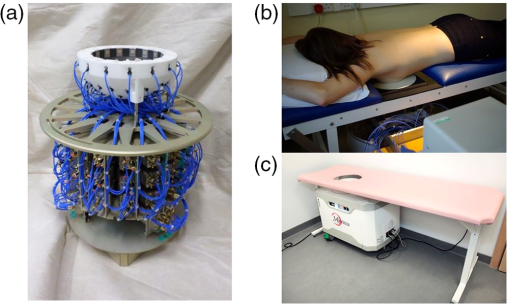
\includegraphics[width=0.5\textwidth]{MARIA_M4.png}
    \centering
    \caption{The MARIA M4 and M5 system. (a) The MARIA M4 antenna array. (b) The M4 in a clinical setting. (c) The integrated M5 package \cite{preeceMARIAM4Clinical2016}}
    \label{fig:MARIAM4}
\end{figure}

\noindent The team scanned 86 participants, with a mean age of 51.4 and a range of 24 - 78 years old. The M4 system showed a sensitivity of
74\% (64/86) when compared with the "gold-standard' of an ultrasound. The "sensitivity" was determined based on the
ability of the M4 system to localize a lesion as it correlated with the location in the ultrasound image. The research
team also divided the group into pre-/peri- and post- menopausal women and found that the sensitivity was 75\% and 73\%
respectively. However, the reliability of these results are called into question when considering the sample size of the
study. Given a sample size of 86, and assuming a normal distribution and that the results are statistically significant
($p < 0.05$, Z = 1.96), a 10.58\% margin of error was calculated. While this may not be enough to conclusively prove
that the M4 system is a viable alternative to Mammograms, it is enough to show promise. With a larger sample size, this
margin of error could be narrowed further.

\subsection{Wavelia}
The second system that was considered was the Wavelia Microwave Breast Imaging System developed by MVG Industries
\cite{moloneyWaveliaMicrowaveBreast2021}. The Wavelia system integrates the imaging system as well as the examination
bed into one complete package (Figure \ref{fig:WaveliaSystem}). The integrated package makes the Wavelia system an
appealing choice for some hospitals, however, its large size may be a barrier to adoption in some facilities where space
is a premium. \hfill \break

\begin{figure}
    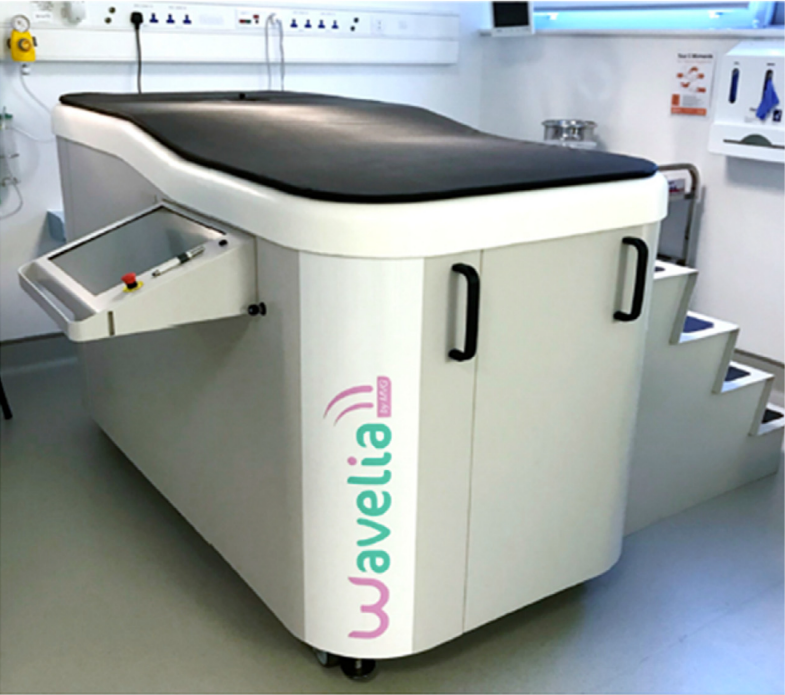
\includegraphics[width=0.5\textwidth]{Wavelia.png}
    \centering
    \caption{The Wavelia System \cite{moloneyWaveliaMicrowaveBreast2021}}
    \label{fig:WaveliaSystem}
\end{figure}

Like in the MARIA M4 system, patients lie in a prone position and place their breasts in the circular cutouts on the
bed. The system then begins to create a 3D reconstruction of the exterior of the breast using a stereoscopic camera.
This also allows for the breast volume to be explicitly calculated rather than being inferred like in the MARIA system.
The Wavelia makes use of the UWB spectrum when imaging the breast, although they opt for a narrower frequency range of
0.5 - 4.0 GHz compared to the 3.0 - 8.0 GHz range of the MARIA system. The antenna configuration, unlike the MARIA system, is an array of 18 Vivaldi-type probes arranged in a concyclic manner
on a horizontal plane. These antennas operate in a Multistatic manner and image the breast in sections parallel to the
coronal plane. The entire antenna assembly moves downwards in 5mm intervals to image the entire breast (Figure \ref{fig:LeveledMultistaticExample}). This is a
leveled multistatic system as opposed to the fully multistatic system in the MARIA M4. This leveled multistatic approach
has the benefit of a theoretically infinite vertical resolution. If the radiologist wanted a finer resolution along the
coronal plane, they would just have to tweak the array vertical step size, rather than having to manufacture an entirely
new antenna array, like in the MERIT system. This leveled approach also allows the parameters of the reconstruction
algorithm to be easily changed based on the particular section of the breast that we are imaging. The fully multistatic
approach, however, would need significant additional logic in the post-processing steps to determine which channels are
coplanar with a particular section. \hfill \break

\begin{figure}
    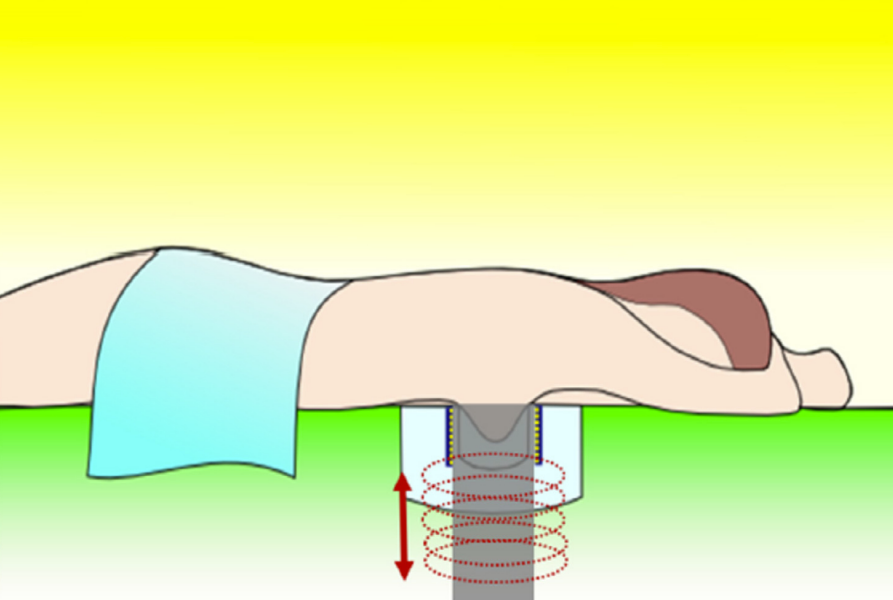
\includegraphics[width=0.5\textwidth]{LeveledMultistatic.png}
    \centering
    \caption{The Leveled Multistatic Approach of Wavelia \cite{moloneyWaveliaMicrowaveBreast2021}}
    \label{fig:LeveledMultistaticExample}
\end{figure}

\noindent The Wavelia paper \cite{moloneyWaveliaMicrowaveBreast2021} conducted a feasibility study on 25 female
participants. While the results aren't statistically significant, they do demonstrate the strengths of the Wavelia
system. 11 of the participants had a biopsy confirmed carcinoma and out of these, the Walia system detected 9 lesions,
with 7 being located to the appropriate region. Overall the system detected an abnormality in 21 of the 24 participants,
leading to a sensitivity of 87.5\%. The researchers do note some limitations of the Walia system, namely it can't detect
any lesions smaller than 10mm. This is significant since the size of the detected lesion plays a big factor when
deciding whether a lesion is cancerous or not. Another limitation of the system is that breast sizes that are too small
cannot be scanned in any great detail by the Wavelia system. Due to the patients being in the prone position, their
breast tissue needs to hang down far enough to have multiple sections of their breast be imaged by the antenna array.
The researchers are working on a subsequent system that should address all the aforementioned limitations. Overall the
participants had a positive outlook on the system. 23 out of the 25 women said that they would recommend the procedure
to other women and all of the women agreed that the information provided was clear and well understood.

\subsection{TSAR}
\setcounter{chapter}{2}
\setcounter{section}{0}
\setcounter{subsection}{0}
\chapter*{Programming Paradigms}
\addcontentsline{toc}{chapter}{Programming Paradigms}
As mentioned in the section before, Julia's development was centered around the philosophy of creating a dynamic yet high
performing language by combining features like Multiple Dispatch and Parametric Polymorphism among others. The following
sections will describe a small subset of these features.

\section{Multiple Dispatch}
Multiple Dispatch is a programming paradigm in which a function can be invoked based not only on the function name but
also on the type and order of input arguments. This is opposed to the single dispatch programming paradigm where the
function dispatched depends on a special argument placed before the function name. In almost all programming languages
this is the variable name for that class. For example, consider the following code: \hfill
\begin{lstlisting}[language=Julia]
# Defined in one library
Class Dog:
    name::string
    function says(a::string):
        print("The dog, $self.name says $a")
    end
end

billy = Dog("Billy")

# Defined in another library
Class Cat:
    name::string
    function says(a::string):
        print("The cat, $self.name says $a")
    end
end

kate = Cat("Kate")
\end{lstlisting}
If one wanted to call the \lstinline[language=Julia]{says} from the Cat or Dog class in the single dispatch paradigm,
one would have to write \lstinline[language=Julia]{billy.says("Hello World")} or
\lstinline[language=Julia]{kate.says("Hello World")}. This concept fits well with object-oriented programming languages
where classes are used to encapsulate concepts. However, a drawback of this system is that the compiler relies on the
user to remember which methods belong to the class and which methods are callable. Also since both the Cat and Dog
classes are defined in different libraries it is not clear how either developer could create a function where these
classes interact with each other without having to create a separate third library that implements compatibility code.

Multiple and its particular implementation in Julia solves some of these issues. In Julia, methods no longer belong to
classes, instead like in C they simply belong to a particular library, also known as a ``Module'' in Julia. Functions
defined in modules are usually exported such that they are available in the namespace of any other module that uses it.
This allows modules to use and overload functions and structures from other modules in a way that is completely
transparent to the end user.   
\begin{lstlisting}[language=Julia]
# Defined in library A
struct Dog{
    name::string
}

function says(pet::Dog, a::string)
    print("The dog, $pet.name says $a")
end  

# Defined in library B 
struct Cat{
    name::string
}

function encounters(petA, petB)
    print("$petA.name encounters $petB.name and $meets(petA, petB)")
end

function meets(petA::Cat, petB::Dog)
    return "hisses"
end

function meets(petA::Dog, petB::Cat)
    return "barks"
end

# Overloading function from library A
function says(pet::Cat, a::string)
    print("The cat, $pet.name says $a")
end


# Someone else using both libraries
billy = Dog("Billy")
kate = Cat("Kate")

says(billy, "Hello World")
says(kate, "Hello World")

encounters(kate, billy)
encounters(billy, kate)
\end{lstlisting}
In the above code block, library B overloads the \lstinline[language=Julia]{says} function to accept a struct of type
Cat. In addition to this, it also creates two new \lstinline[language=Julia]{meets} functions that handle the
interaction between the Cat and the Dog types, as well as an \lstinline[language=Julia]{encounters} function. A third
user can make use of both libraries as they did in the single dispatch case, but now they only have to call the function
name, rather than the function name prepended with the class variable name. In the case of the
\lstinline[language=Julia]{says} function call, the Julia compiler automatically dispatches the correct implementation
based on the type of the input argument. This is further exemplified in the final two function calls. As stated before
multiple dispatch is sensitive to both the type and order of the inputs. In the first call to the
\lstinline[language=Julia]{encounters} function, the \lstinline[language=Julia]{meets} function on line 19 will be
dispatched as the argument order was of type Cat and then Dog. Whereas in the second call to the
\lstinline[language=Julia]{encoutners} function, the \lstinline[language=Julia]{meets} function defined on line 23 will
be dispatched due to the reverse ordering of the types.

\begin{figure}[!h]
    
\includegraphics[width=1\textwidth]{multipleDispatch.png}
    \centering
    \caption{Multiple Dispatch (top) vs Single Dispatch (bottom) demonstrating that in the multiple dispatch paradigm, the executed function also depends on the type and order of its inputs} 
    \label{fig:multipleDispatch}
\end{figure}

\section{Type Heirarchy}
In Julia, all types are arranged in a tree-like structure and can be broadly classified into two categories, an Abstract
Type or a Concrete Type. Abstract types are the internal nodes of the type tree, having both parents and children, while
concrete types are the ``leaves'' of the tree, having parents but no children. Another notable difference between
abstract types and concrete types is that abstract types cannot be instantiated, they serve only as nodes in the type
graph. Shown in Figure \ref{fig:juliaTypeHeirarchy}, is the type hierarchy for the Integer type, abstract types are
highlighted in red, whereas concrete types are highlighted in blue. \hfill
\begin{figure}[t]
    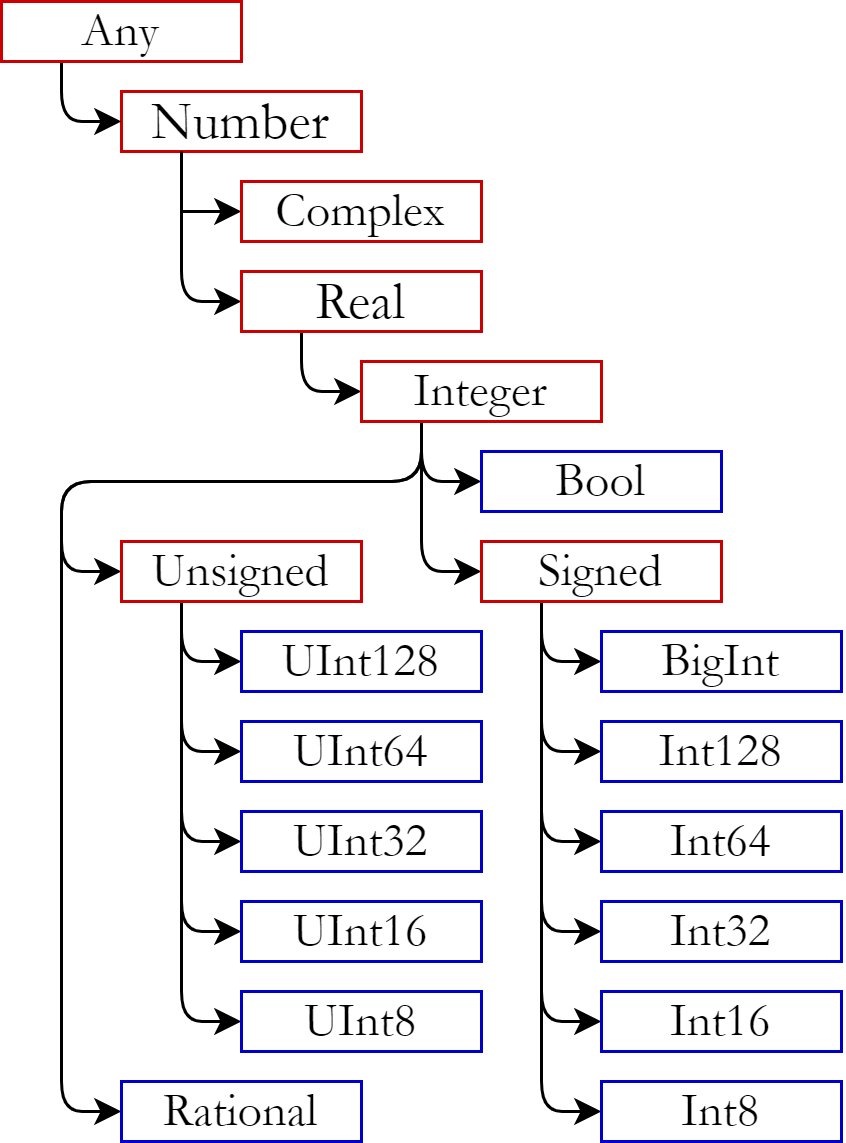
\includegraphics[width=0.45\textwidth]{juliaTypeTree.png}
    \centering
    \caption{Type hierarchy for the Integer Type} 
    \label{fig:juliaTypeHeirarchy}
\end{figure}
\FloatBarrier
The type hierarchy not only provides a way to logically organize types but also tightly integrates with the multiple
dispatch system mentioned before. It is this pairing that allows Julia to fulfill its promise of easy and powerful
extensibility. The following example helps illustrate this further.
\begin{lstlisting}[language=Julia]
# Defined in library A
abstract type Animal end

struct Cat <: Animal
    name::string
end

struct Dog <: Animal
    name::string
end

function encounters(petA::Animal, petB::Animal)
    verb = meets(petA, petB)
    println("$(petA.name) meets $(petB.name) and $(verb)")
end

meets(petA::Animal, petB::Animal) = "passes by."
meets(petA::Cat, petB::Dog) = "hisses"
meets(petA::Dog, petB::Cat) = "barks"

# Defined in library B
struct Rabbit <: Animal
    name::String
end

whiskers = Cat("Whiskers")
chomper = Rabbit("Chomper")
encounters(whiskers, chomper)
\end{lstlisting}
Library A defines a type hierarchy with Cat and Dog being a subtype of the abstract Animal type. The library then
implements a series of \lstinline[language=Julia]{meets} functions and an \lstinline[language=Julia]{ecounters}
function, similar to the example in the previous section. However, unlike the example before, there is a new
\lstinline[language=Julia]{meets} which accepts an argument of type Animal. Library B, importing library A, defines a
Rabbit type that is a subtype of the Animal abstract type and then calls the encounters function from library A. The
dispatch system cannot execute the \lstinline[language=Julia]{meets} function from lines 18, since
\lstinline[language=Julia]{chompers} is not of type Dog. Instead, it executes the \lstinline[language=Julia]{meets}
function on line 17, since both \lstinline[language=Julia]{whiskers} and \lstinline[language=Julia]{chompers} are valid
Animal types. This highlights an important interplay between the type hierarchy and the multiple dispatch system, in
that when dispatching, the Julia compiler will select the function that is most specific across all its input arguments.
The developer of library A need not worry about all the other possible Animal types, or what their fields may contain,
they can create a generic \lstinline[language=Julia]{meets} function that accepts any subtype of the Animal class and
will execute successfully provided the subtyped class contains the fields being accessed. Neither developer has to worry
about the completeness of the other's implementation, provided developer B follows the standards set by developer A,
they can develop an extension to library A and trust that the two libraries will be comparable.

\section{Parametric Polymorphism}
Parametric polymorphism refers to the programming paradigm where a function can be made generic to the input argument
type. At compilation time, the compiler can strongly type the function based on the types of the input arguments.
Consider the simple example of an \lstinline[language=Julia]{addtwo(x)} function.
\begin{lstlisting}[language=Julia]
function addTwo(x::T) where {T <: Real}
    return x + T(2)
end
\end{lstlisting}
Instead of specifying a concrete type for \lstinline[language=Julia]{x}, it is parametrized by the variable
\lstinline[language=Julia]{T} which has an abstract type restriction on it. This implies that
\lstinline[language=Julia]{T}, and by extension \lstinline[language=Julia]{x}, can by any type that is a subtype of the
Real abstract type. If parametric polymorphism was not a Julia feature, this function would have to be duplicated 16
times to account for the various concrete types that are a subtype of Real (see Figure \ref{fig:juliaTypeHeirarchy}).

\section{Type Stability}
\label{TypeStability}
Type Stability is a coding discipline that Julia recommends all code use. A function whose contained variables have a
consistent type for its lifetime is considered to be ``type stable'' or to have ``type stability''. Another way to think
about this, is that if the output type depends only on the input types, then the function is type stable. Consider the
following two functions: 
\begin{lstlisting}[language=Julia]
function unstable()
    x = 1
    for i = 1:10
        x /= rand()
    end
    return x
end

function stable()
    x = 1.0
    for i = 1:10
        x /= rand()
    end
    return x
end
\end{lstlisting}
Both functions have a variable, \lstinline[language=Julia]{x} which is divided 10 times by random floats and is returned
at the end of the function. However, based on the description above, the first function is considered to be ``Type
Unstable'' whereas the second function is considered to be ``Type Stable''. This is because in the first function the
type of \lstinline[language=Julia]{x} changes in the lifetime of the function (turns from Int64 to Float64). However in
the second function, the data type of \lstinline[language=Julia]{x} stays as a Float64 throughout the lifetime of the
function. The notion of type stability is important as it allows the Julia compiler to perform optimizations based on
the known data type of the variables at compile time. For type unstable functions, their unstable variables default to
type Any, ergo forgoing any optimizations. These optimizations are evident when benchmarking the functions above. This
was performed using the \lstinline[language=Julia]{@benchmark} macro from the BenchmarkTools module. Both functions were
run multiple times to ensure that only the compiled versions of the functions were executed rather than the interpreted
version. These benchmarks showed that on average the type unstable function ran 1.87x slower than the type stable
function (573.355ns and 306.178ns respectively).  

\section{Closure}
Closure in programming refers to the practice of calling a function A that returns a function B which has some
information about the variables contained in the scope of function A. Consider the following simple example:
\begin{lstlisting}[language=Julia]
function addX(x)
    scalar = x
    function calc_(a)
        return a + scalar
    end
end

add5 = addX(5)
add7 = addX(7)

add5(2)  # Will return 7
add7(10) # Will return 17
\end{lstlisting}
Defined above is a function called \lstinline[language=Julia]{addX} which accepts an input \lstinline[language=Julia]{x}
and assigns it to a variable \lstinline[language=Julia]{scalar}, before constructing and returning the function
\lstinline[language=Julia]{calc_}. This can be beneficial as it allows developers to create a family of functions that
are parametrized by their input variable.  It must be noted that the
captured variable, in the above case \lstinline[language=Julia]{scalar}, must never be reassigned, otherwise, the
compiler will not be able to infer the data types leading to type unstable code, and by extension all the negative
consequences mentioned in the previous section.

\section{Type Safety}
Type Safety refers to a program or language's ability to detect and discourage errors that arise from performing
operations on the wrong data type. For example in Julia, it is simple to add two numeric types, but performing the same
operation on two strings would yield an error, since the summation operator is not defined for two string types. This
offers some level of protection against illegal operations, but there are many cases where the type of the variables
agree with the operation being performed, but their semantic meaning disagrees. The example below will illustrate this
idea.
\begin{lstlisting}[language=Julia]
function calcSpeed(dist::Vector{T}, t::Vector{T}) where {T <: Real}
    return dist ./ t
end

#################################################### 
distance = rand(1, 100)
time = rand(1, 100)
calcSpeed(distance, time)   # Will compute the speed

#################################################### 
distance = rand(1, 100)
time = rand(ComplexF64,1, 100)

# Will throw an error since there is a type mismatch
calcSpeed(distance, time)  

#################################################### 
distance = rand(1, 100)
time = rand(1, 100)

# Will compute the wrong answer, but no error gets thrown
calcSpeed(time, distance) 
\end{lstlisting}
In the code block above \lstinline[language=Julia]{calcSpeed} accepts a vector of distance and time and returns the
associated speeds. Executing line 8, as expected returns the calculated speeds correctly. Executing line 12 will throw a
type error since ComplexF64 is not a subtype of Real. Line 22 however, will execute and return successfully even though
the wrong answer is returned, as the arguments were provided in the wrong positional order. This is because compilers
can only make inferences regarding the legality of a statement based solely on the concrete types of its arguments
rather than their semantic meaning in the context of the function being executed. However, the chance of variables being
incorrectly passed positionally can be negated by creating lightweight types that encode this semantic information in
their type name. In the above case, it would mean creating a ``distance'' type and a ``time'' type that act as wrappers
around a numerical concrete type. This way when line 22 is executed, instead of returning an incorrect answer, the
compiler will raise an error as the ``time'' and ``distance'' types were provided in the wrong order.
\setcounter{chapter}{3}
\setcounter{section}{0}
\setcounter{subsection}{0}

\chapter*{Julia For Development}
The features mentioned in the previous chapter are extensively used in the 10,760 packages currently being hosted on
JuliaHub and the Julia Package Manager. The following sections will contextualize the role that Julia and its features
play in the broader field of scientific computing as well as its role in MERIT.jl. 

\section{Julia For Scientific Computing}
Julia and its libraries are an attractive choice for researchers in the fields of numerical analysis, data science and
engineering. Consider the common task of solving differential equations. These equations, defined in terms of
derivatives, underpin every field of engineering from the analysis of complex electronic systems to thermodynamical
systems. The Julia package DifferentialEquations.jl \cite{rackauckas2017differentialequations} allows users to define
and solve differential equations in as little as six lines of code. Consider the example below:
\begin{lstlisting}[language=Julia]
using DifferentialEquations
f(u, p, t) = 1.01 * u
u0 = 1 / 2
tspan = (0.0, 1.0)
prob = ODEProblem(f, u0, tspan)
solution = solve(prob)
\end{lstlisting}
After defining the differential equation, initial conditions and the solution time length, the example defines an
\lstinline[language=Julia]{ODEProblem} which is a subtype of \lstinline[language=Julia]{SciMLBase.AbstractODEProblem} which
itself is subtyped from \lstinline[language=Julia]{SciMLBase.AbstractDEProblem} and this pattern continues. Notice that
the abstract type for ODEProblem was defined in the SciMLBase Module, not in the DifferentialEquations Module. SciMLBase
is a separate library that DifferentialEquations extends in a way that is completely transparent to the end user. Any
problems created using the ODEProblem type from DifferentialEquations can be used in any function from any library that
can accept the SciMLBase.AbstractODEProblem or any of its supertypes. This highlights how easy it is for new libraries
to extend older libraries in a way that is mutually beneficial for both libraries. The developer of the original library
no longer has to worry about implementing functions for every type of differential equation, and the developer of the
new library does not have to invest time in creating the complex type hierarchy or the helper functions from the
original library. Once passed to the \lstinline[language=Julia]{solve} function, the library can automatically determine
the best solver based on the problem and dispatch the relevant methods accordingly exemplifying the use of multiple
dispatch, all while boasting C and Fortran-like speeds. Their webpage demonstrates them solving the Lorenz ODE in
789.794~$\mu$s. Julia also has libraries for the field of Biology such as, but not limited to, JWAS.jl for whole genome
analysis, BioStructures.jl for manipulating macromolecules, VarientVisualization.jl for visualizing genomic variation
data and Gillespie.jl for Gillespie-type simulations in Julia. In the field of Machine Learning, there are various
libraries such as Flux.jl and TensorFlow.jl as generic machine learning libraries, BrainFlow.jl for EEG, EMG and ECG
data, and NeuralNetDiffEq.jl for physics-informed neural networks, to name a few. The easy extensibility and intuitive
interfaces that can be created using the language features in Julia make it an attractive language for developers
creating libraries and researchers who want quick answers to their questions. 

\section{Julia for MERIT.jl}
MERIT.jl also makes full use of the aforementioned features in order to create a library that is reliable, performant
and easily extensible. The sections below will outline how each feature was used to attain the goals stated at the begining.  

\subsection{Multiple Dispatch in MERIT.jl}
MERIT.jl makes use of multiple dispatch in the beamforming algorithm implementations. As mentioned before, the DAS
beamformer can be considered as a specialized case of the WDAS algorithm with a constant unit weighting factor. Due to
both being effectively the same algorithm, it was decided to combine both of these under the DAS nomenclature and use
multiple dispatch to select the correct function based on the presence of weighting factors in the argument list. This
was also used when defining the addition, subtraction and exponentiation operators so that the users can make use of the
inbuilt mathematical operators when working with the Point3 and Point2 datatypes. Multiple dispatch could also be used
in the implementation of the time domain version of the DAS beamformer, the specifics of which will be detailed in
section \ref{TDImplementation}.  

\subsection{Type Hierarchy in MERIT.jl}
The concept of abstract types and subtypes is used heavily in MERIT.jl due to the constant pace of progression in the
field. Currently, most of the research in microwave imaging is centered around breast imaging and breast cancer, however
in 2013, a pilot study published in the International Journal of Biomedical Imaging found the use of microwave imaging
to be beneficial when imaging transverse sections of the forearm \cite{gilmoreMicrowaveImagingHuman2013}. As such the
library needs to be flexible enough to adapt to novel imaging domains. The type hierarchy in MERIT.jl is centered around
the Scan abstract type, from this, the BreastScan type is subtyped which holds all the information regarding the scan
from a particular breast. In order to incorporate the aforementioned study, one would have to create a ForearmScan type,
subtyped from Scan, which has a similar field name structure to the BreastScan type. In this way, MERIT.jl achieves
extensive flexibility and expandability which would not be possible in other languages.
\begin{figure}[h!]
    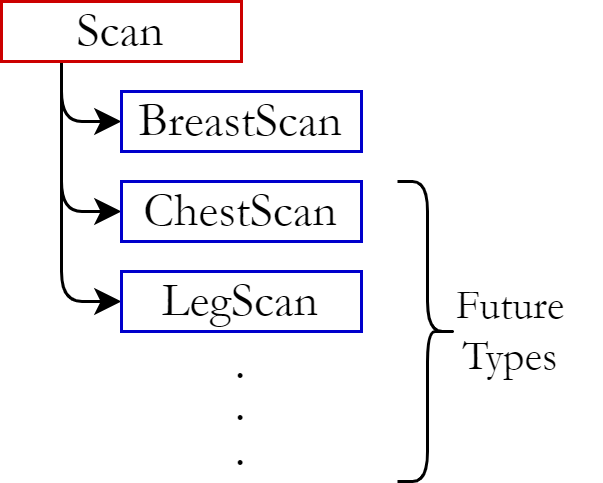
\includegraphics[width=0.5\textwidth]{scanType.png}
    \centering
    \caption{Current type hierarchy in MERIT.jl} 
    \label{fig:scanType}
\end{figure}
\FloatBarrier
This type hierarchy also synergizes with the multiple dispatch feature in Julia. Since the algorithms in MERIT.jl are
not specific to a particular body part, the one-call processing pipeline demonstrated in section \ref{CurrentWorkflow}
could easily be extended to work with any type that subtypes the Scan type, provided that the new type has a similar
field name structure to the current BreastScan struct. Full details surrounding the structure of the BreastScan struct
can be found in the Scans.jl file.


%% COULD GO IN RESULTS
% \begin{lstlisting}[language=Julia]
% function delay_template(relative_permiativity)
%     # Capture the relatively_permiativity
    
%     # Create a delay function
%     function calc_(channels, antenna, domain_points):
%         #calculate and return a time matrix
%         #Size = (1 x #Channels x #Points)
%     end
% end

% function beamformer(delayed_signals)
%     #Do some processing
%     #return should be of size (1 x 1 x #Points)
% end
% \end{lstlisting}
% These templates allow for a lot of flexibility and are really where MERIT.jl shines in comparison to its MATLAB
% counterpart. Researchers who just want to benchmark new algorithms against already established ones just need to follow
% these templates and they can be guaranteed that their functions will ``just work'' with the one-call data processing
% pipeline. If their functions also follow the rules of type stability mentioned in previous sections, they can also have
% some reasonable guarantees that any slowdowns are caused by their implementations rather than the lack of compiler
% optimizations for type unstable code.

\subsection{Parametric Polymorphism in MERIT.jl}
MERIT.jl makes use of parametric polymorphism so that the functions it implements can be agnostic to the data type of
its inputs. When instantiating the BreastScan struct the user can provide the types of the data that will be loaded and
can therefore set the internal data type of the struct. It would be impossible to support all 4,176 different
permutations of every type pairing, however, with parametric polymorphism, each function only needs to be defined once
and the Julia compiler will handle the rest. This means that researchers and developers don't have to worry about
whether the library functions can support the data type of their data, so long as it follows the type restriction set on
the function, it will produce an output, creating an intuitive and easy coding experience. 

\subsection{Type Stability in MERIT.jl}
As shown in section \ref{TypeStability}, the performance gained by writing type stable code can be significant. These
gains become important when considering the many millions of function calls required to generate an output in MERIT.jl.
Consider just the distance calculations required between an $8$~cm radius breast whose domain is discretized with a
resolution of $0.25$~cm and an antenna array made of 60 antennas; this equates to roughly 4.2 million calculations alone
for each image. Performing this on a type unstable function would take far too long to compute, rendering the library
unusable. Herein lies one of the drawbacks of writing Julia code, namely, the ease at which an inexperienced developer
can write type unstable functions. In the simple case in section \ref{TypeStability}, the cause for the type instability
is evident, however, with larger more complex functions it can be hard to narrow down the cause for the instability. The
language does however, offer the \lstinline[language=Julia]{@code_warntype} macro that can analyze sections of code and
indicate, but not fix, places of instability where the compiler fails to infer the data type of the variable. This tool
can considerably benefit developers of MERIT.jl to ensure that any extensions written for the language align
with its philosophy of performance.

\subsection{Closure in MERIT.jl}
Closure, in MERIT.jl, was the programming paradigm that was used in order to achieve some customizability for the
functions that required it. Currently, it is being used in the \lstinline[language=Julia]{get_delys} in the Breamform.jl
file. Earlier sections showed how $\varepsilon$ is a free parameter in the beamforming equations, one that researchers
would be changing frequently to find the optimal parameter for each particular scan. This allows researchers to quickly
create a set of parametrized delay functions that can be easily interpolated into the BreastScan struct to be used in
the one-call processing pipeline, allowing them to answer questions regarding the optimal range for $\varepsilon$
depending on the body part or tissue composition.

\subsection{Type Safety in MERIT.jl}
The MERIT.jl library exemplifies the idea of ``strong'' type safety through its implementation of the Point data type.
The Point type is an abstract type from which the Point3 and Point2 concrete type subsets. These are lightweight
wrappers around a grouping of 3 and 2 numerical types respectively and serve the purpose of being a 3D and 2D point.
\begin{lstlisting}[language=Julia]
abstract type Point end

# xyz can be any data type that is a subset of Real
mutable struct Point3{T <: Real} <: Point
    x::T
    y::T
    z::T 
end

mutable struct Point2{T <:  Real} <: Point
    x::T
    y::T
end
\end{lstlisting}
Due to the custom nature of these data types, the inbuilt operators could not be used on them. So in addition, MERIT.jl
had to extend the in-built operators using the concepts of multiple dispatch and parametric polymorphism as mentioned
before such that these types could be useful. The full suite of implemented operators can be found in the GitHub
repository. Every function in the library that needs to work with points accepts a collection of a Points subtype
rather than a collection of numbers. This way no other collection of numbers can be erroneously passed in place of the
Points subtypes. Some edge cases still exist however, there is nothing stopping a user from incorrectly passing a
collection of points describing antenna locations to an argument which is for points from the imaging domain. Even
though this issue still exists, clear and easy to understand documentation should make this a nonissue. It should be
noted that in its current state, MERIT.jl is not completely strongly typed, this is an area of the library which can be
improved upon in the future. 

\setcounter{chapter}{4}
\setcounter{section}{0}
\setcounter{subsection}{0}
\chapter*{Results}
\addcontentsline{toc}{chapter}{Results}
\section{Current Workflow}
\label{CurrentWorkflow}
The current workflow in MERIT.jl was designed to be simple and approachable without much background knowledge about how
Julia or the underlying library works. Shown below is the full workflow needed to generate a plot from the data:
\lstinputlisting[language=Julia]{../../src/GettingStarted.jl}
A user would first instantiate the BrestScan struct and assign the data types that would be used throughout the
processing pipeline. The first type sets the data type and thereby the precision of the points composing the imaging
domain, the antenna locations and the frequency divisions. This can be any datatype that is a subset of type Real. The
second type controls the data type of the signal matrix containing the data collected from each antenna. This can be any
type that is a subtype of Number allowing for time-domain (Real) signals or frequency-domain (Complex) signals. The
third type controls the data type of the channels, and it can be any type that is a subtype of Integer. The choice of
data type here has no accuracy impact on the final result and it is recommended to choose an Unsigned Integer data type
that is big enough to index all the antennas. The next step would be to generate the imaging domain, this is
accomplished using the \lstinline[language=Julia]{domain_hemisphere!} function. This accepts the resolution and the
assumed or calculated radius of the breast. The user would then have to make use of the
\lstinline[language=Julia]{load_XXX!} functions to load the data into the relevant fields of the struct. These functions
assume the data is contained in a CSV file and contain no headers. The user then populates the relevant fields with
their chosen beamformer and delay function. At this stage, the user can then pass the whole struct to the
\lstinline[language=Julia]{beamform} which will beamformer the provided signals into a set of data that can then be
visualized as demonstrated towards the end of the code block above. Overall the entire workflow can be seen in Figure
\ref{fig:MERITWorkflow}.

\begin{figure}[h!]
    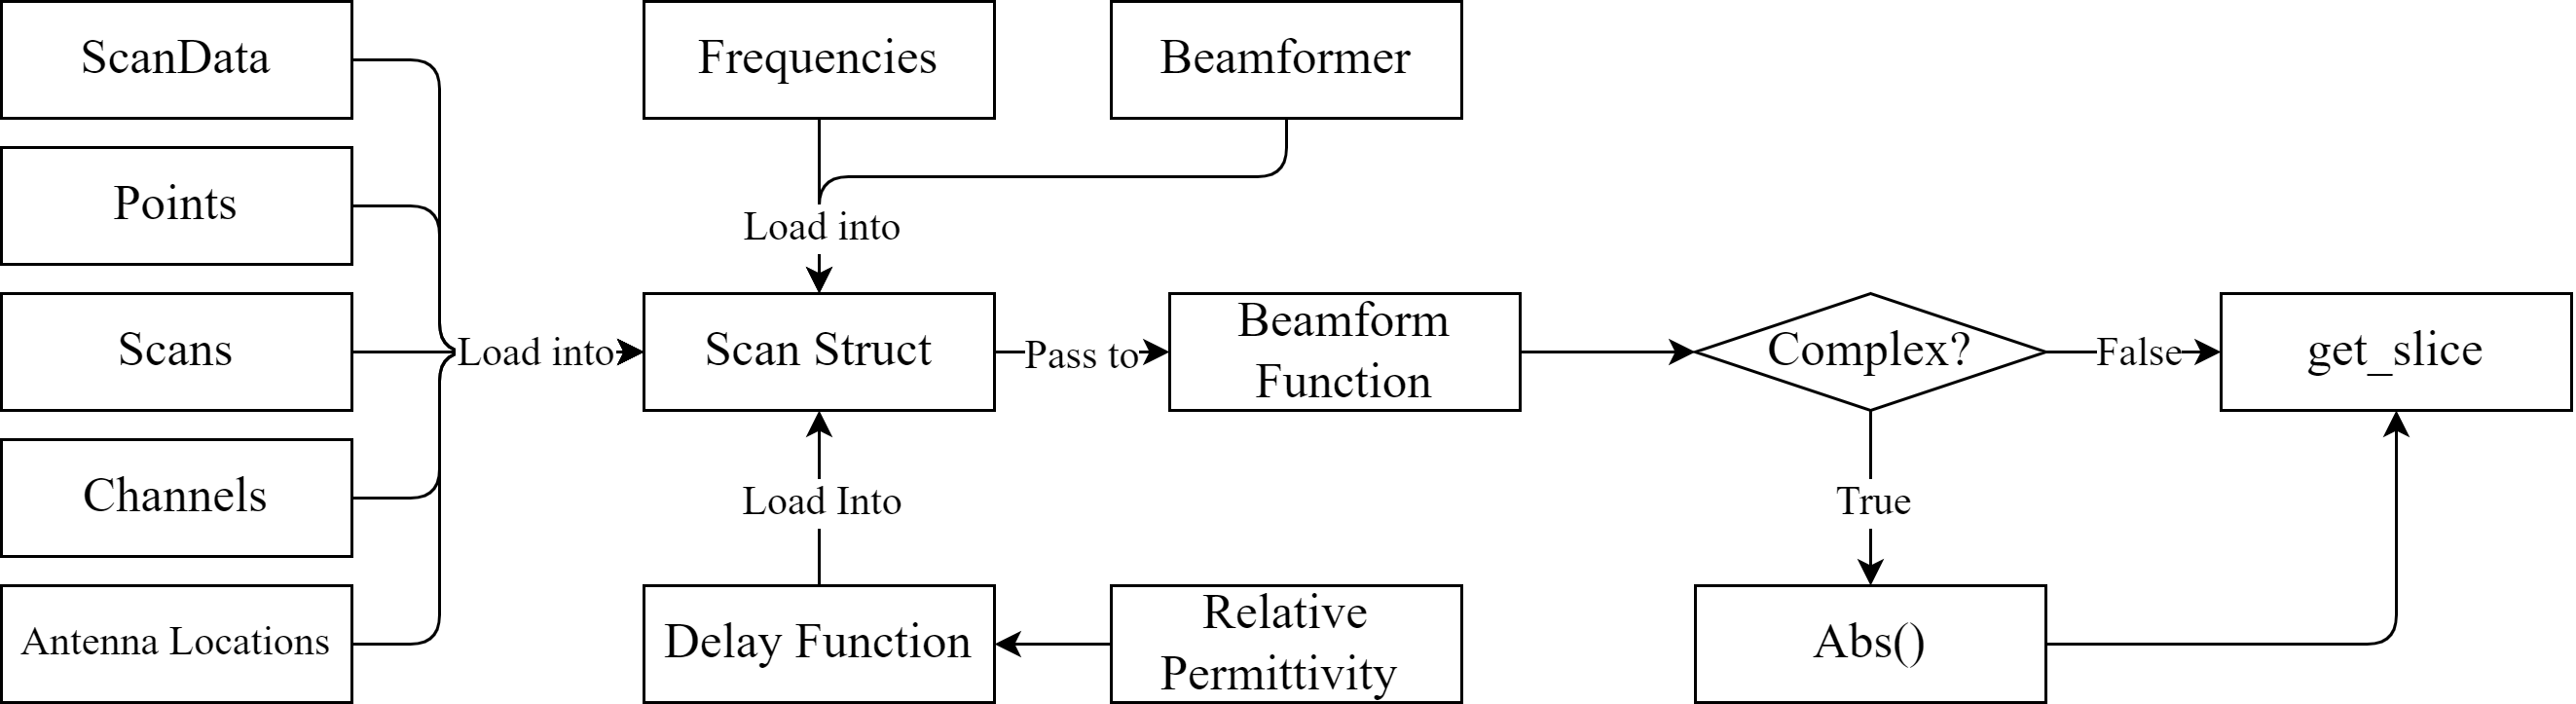
\includegraphics[width=1\textwidth]{MERITWorkflow.png}
    \centering
    \caption{An overview of the current workflow used to image a scan in MERIT.jl} 
    \label{fig:MERITWorkflow}
\end{figure}

This workflow exemplifies how easy it is to use the MERIT.jl library. The function names were deliberately chosen to be
verbose and conform to established nomenclature in the field so that anyone who wants to use the library can understand
what each function does without having to delve into the source code. In this way, the MERIT.jl library is somewhat self
documenting. Additional information is provided above each function in the form of docstrings which can be used with the
help function built into the Julia REPL. This was done in a bid to lower the prerequisite knowledge needed to use the
library, thereby fulfilling one of the goals of MERIT.jl which was to create an open and accessible library. 

\section{MERIT.jl Results}
The library was benchmarked against the MATLAB implementation created by Dr. O'Loughlin \textit{et al.} to ensure that the
results provided by MERIT.jl are provably correct. Both implementations were given the same data, B0\_P3\_p000.csv and
B0\_P3\_p036.csv. Rotational subtraction was performed on these in both libraries to reduce the presence of skin
reflections in the data as mentioned before. The data was then processed according to the processing pipeline
recommended by both libraries, the result of which can be seen below in Figure \ref{fig:OutputResults}. It should be
noted that the \lstinline[language=Octave]{imshow} function was used in MATLAB to plot the image. This had the effect of
reflecting the image across the x-axis and also slightly stretching the image along the x-axis, however, the matrix
holding the image data still shares the same layout as the image matrix in Julia so a numerical comparison between the
two could be performed. The averaged MSE proved to be an excellent choice as a numerical comparator, due to the squaring
operations in the MSE formula any small differences would be greatly magnified in the error. This is desirable when the
goal is to see if MERIT.jl can provide output that is similar to its MATLAB counterpart. Computing the averaged MSE
between the two images yielded an error of $8.4417 \times 10^{-7}$ which is well within the accuracy of a float, making
it effectively identical to the images produced by MATLAB. This shows that the Julia library in its current state
provides a viable alternative to the MATLAB implementation for frequency domain analysis.

\begin{figure}[t]
    \begin{tabular}{cc}
        \subfloat[MERIT.jl Output]{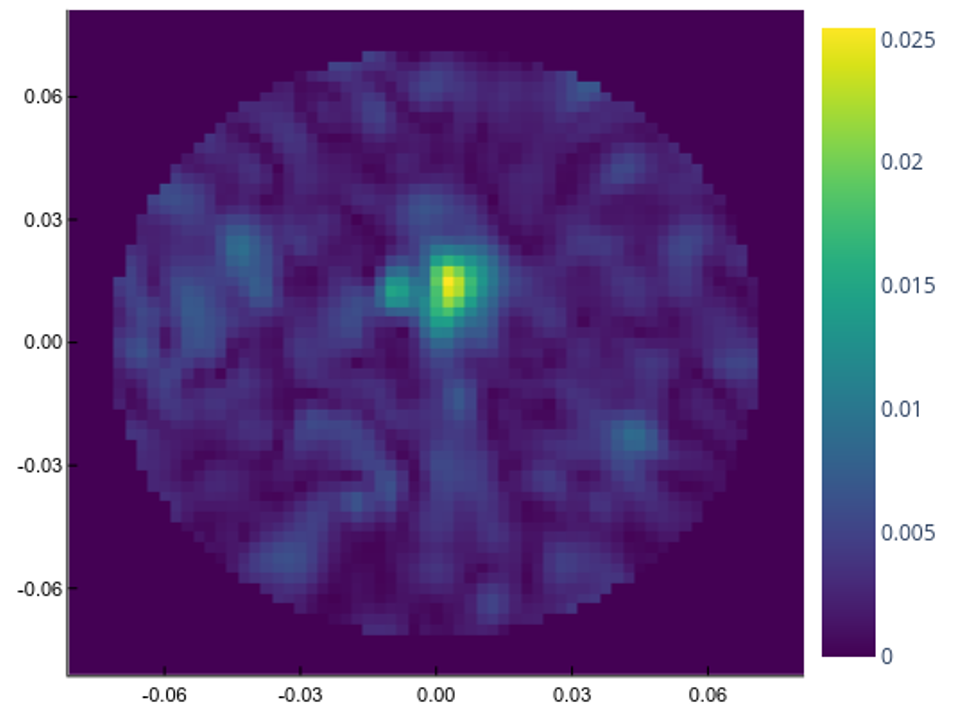
\includegraphics[width=0.45\linewidth]{JuliaOutput.png}}&
        \subfloat[MATLAB Output]{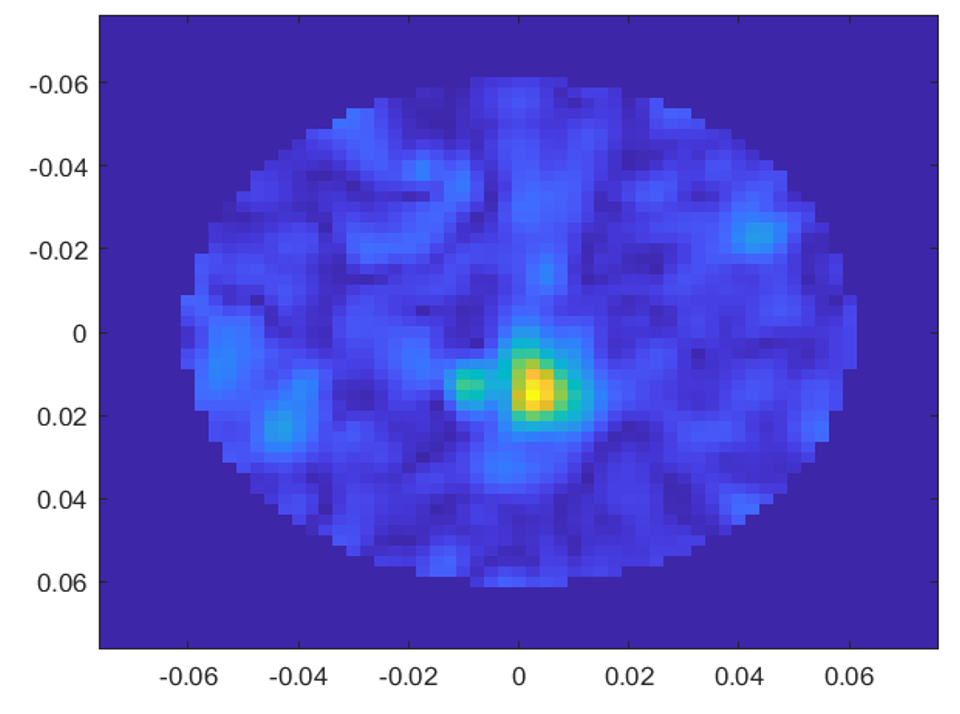
\includegraphics[width=0.45\linewidth]{MATLABOutput.png}}
    \end{tabular}
    \caption{A comparison between Julia and MATLAB output, showing an averaged MSE of $8.4417 \times 10^{-7}$}
    \label{fig:OutputResults}
\end{figure}

\section{Performance of MERIT.jl}
One of the requirements for MERIT.jl was that it had to be performant. Through the use of type stability, SIMD optimized
for loops and the disabling of array bounds checking, the library could process the provided data in 8 seconds. However,
after the addition of the Points data type for type safety, the processing time climbed to 12 seconds. While the overall
runtime is still acceptable, an increase of 3 seconds is less than ideal. While no official analysis has been conducted
to narrow down the cause of the slowdowns, I suspect that perhaps it may be down to unoptimized implementations of the
basic operators such as addition and squaring in the Points.jl library. It should also be noted that when running the
library, my laptop constantly ran into memory limits and had to write some memory to a swap file on disk. I believe that
moving memory in and out of this file might also be partly responsible for the increased runtime, however, further
research is necessary to determine a definitive cause. To capture the full performance characteristics of the library, a
scalability test was performed, in which the number of points, channels and frequency divisions were progressively
increased. This was performed in an automated manner using the functions provided by BenchmarkTools.jl
\cite{BenchmarkToolsJl}. The results from the benchmark suites were then exported to CSV files and analyzed in Excel to
judge the ``Big O'' notation of MERIT.jl.

\begin{figure}[h!]
    \begin{tabular}{cc}
        \subfloat[Raw Points]{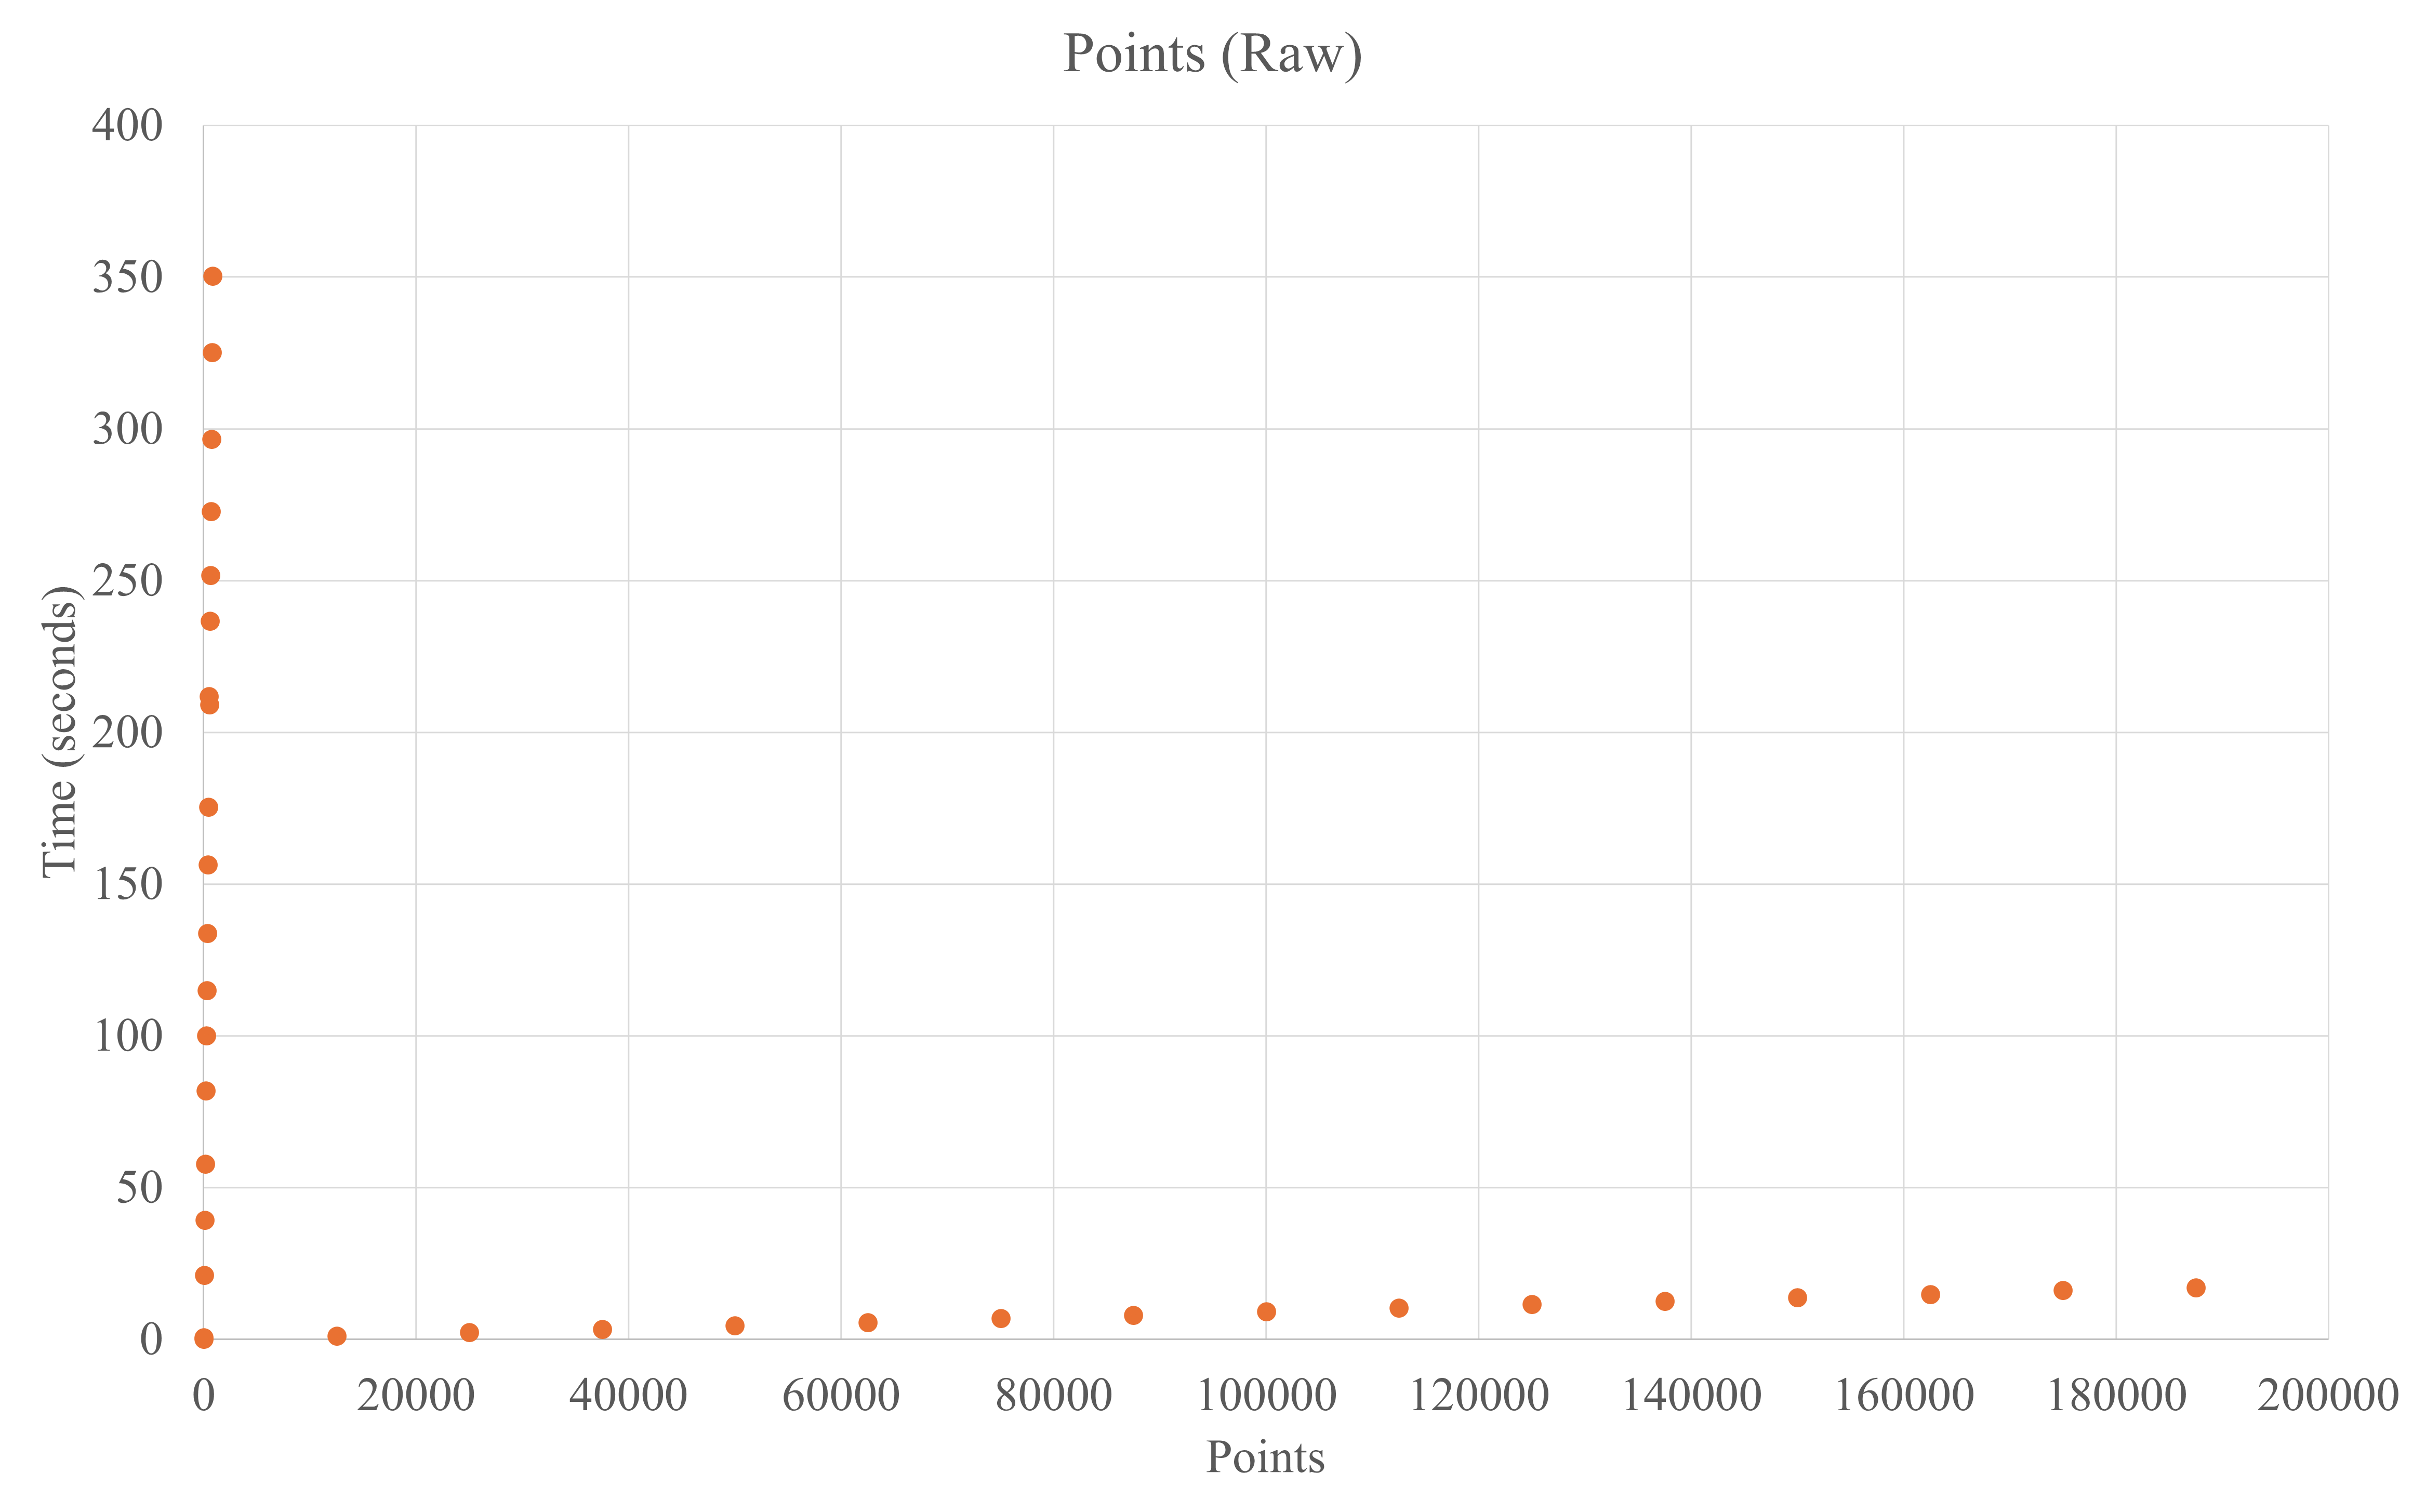
\includegraphics[width=0.45\linewidth]{PointsUnedited.png}}&
        \subfloat[Processed Points]{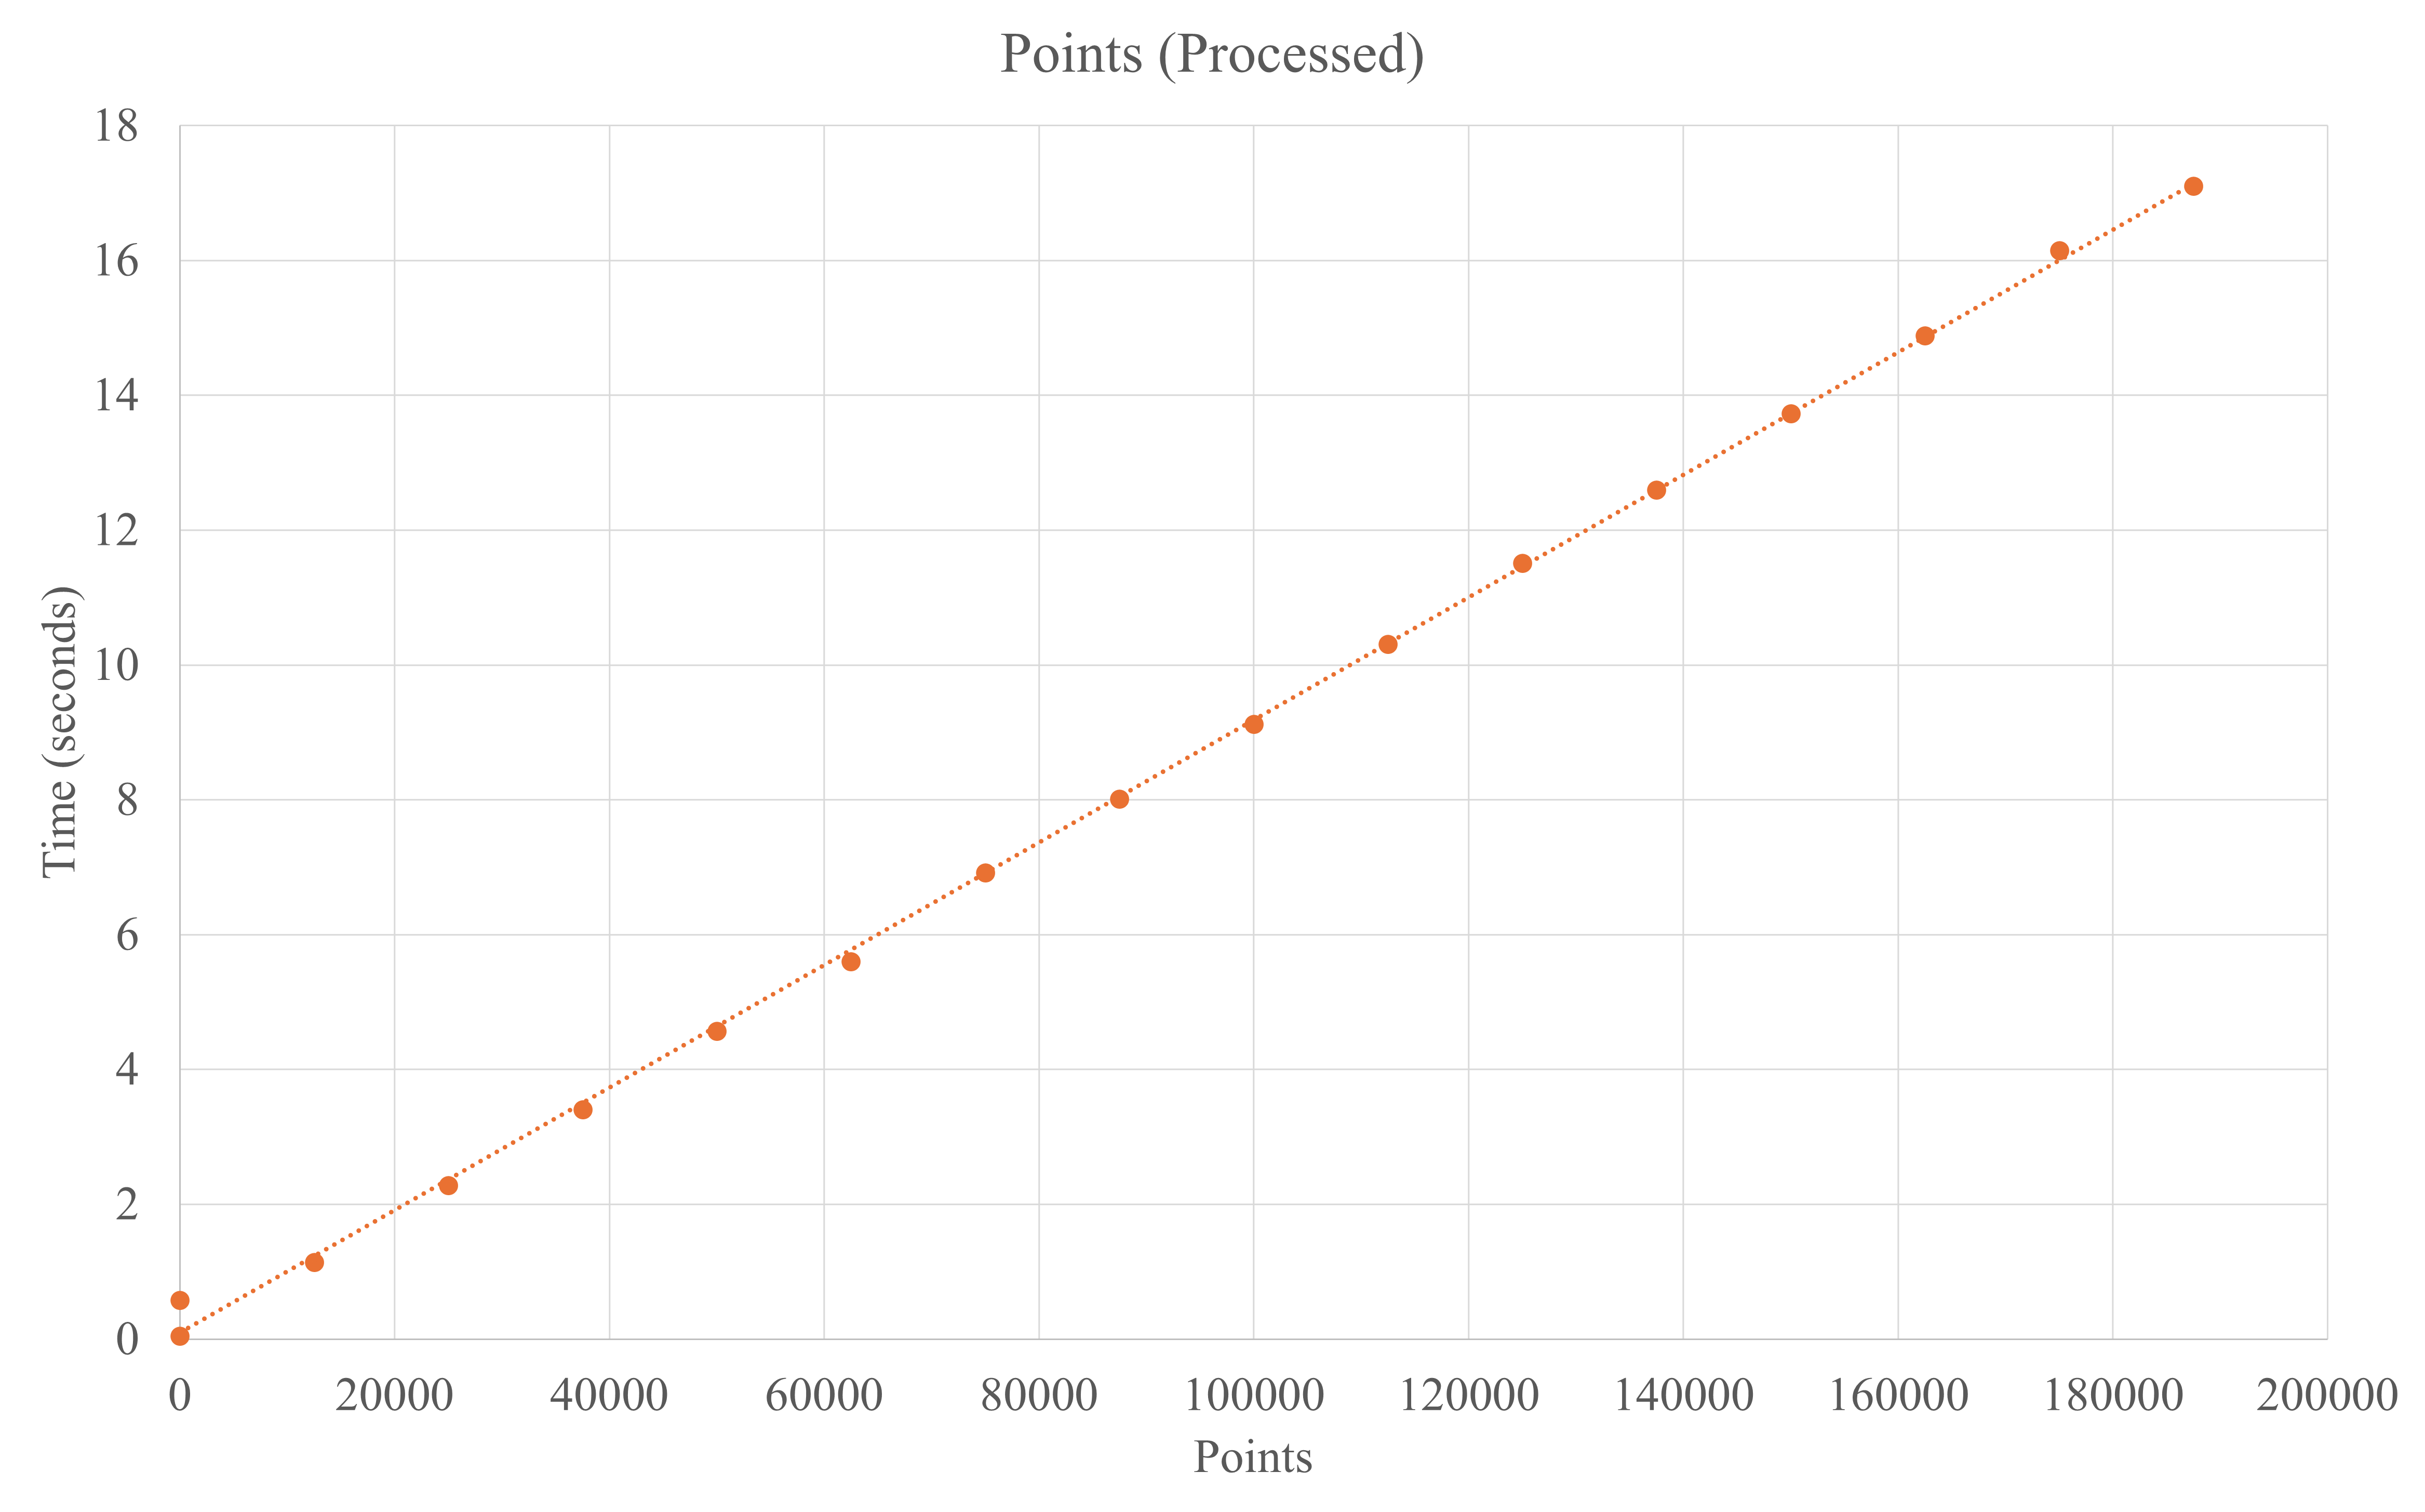
\includegraphics[width=0.45\linewidth]{PointsEdited.png}}
    \end{tabular}
    \caption{Runtime for increasing Points}
    \label{fig:PointsResults}
\end{figure}

\begin{figure}[h!]
    \centering
    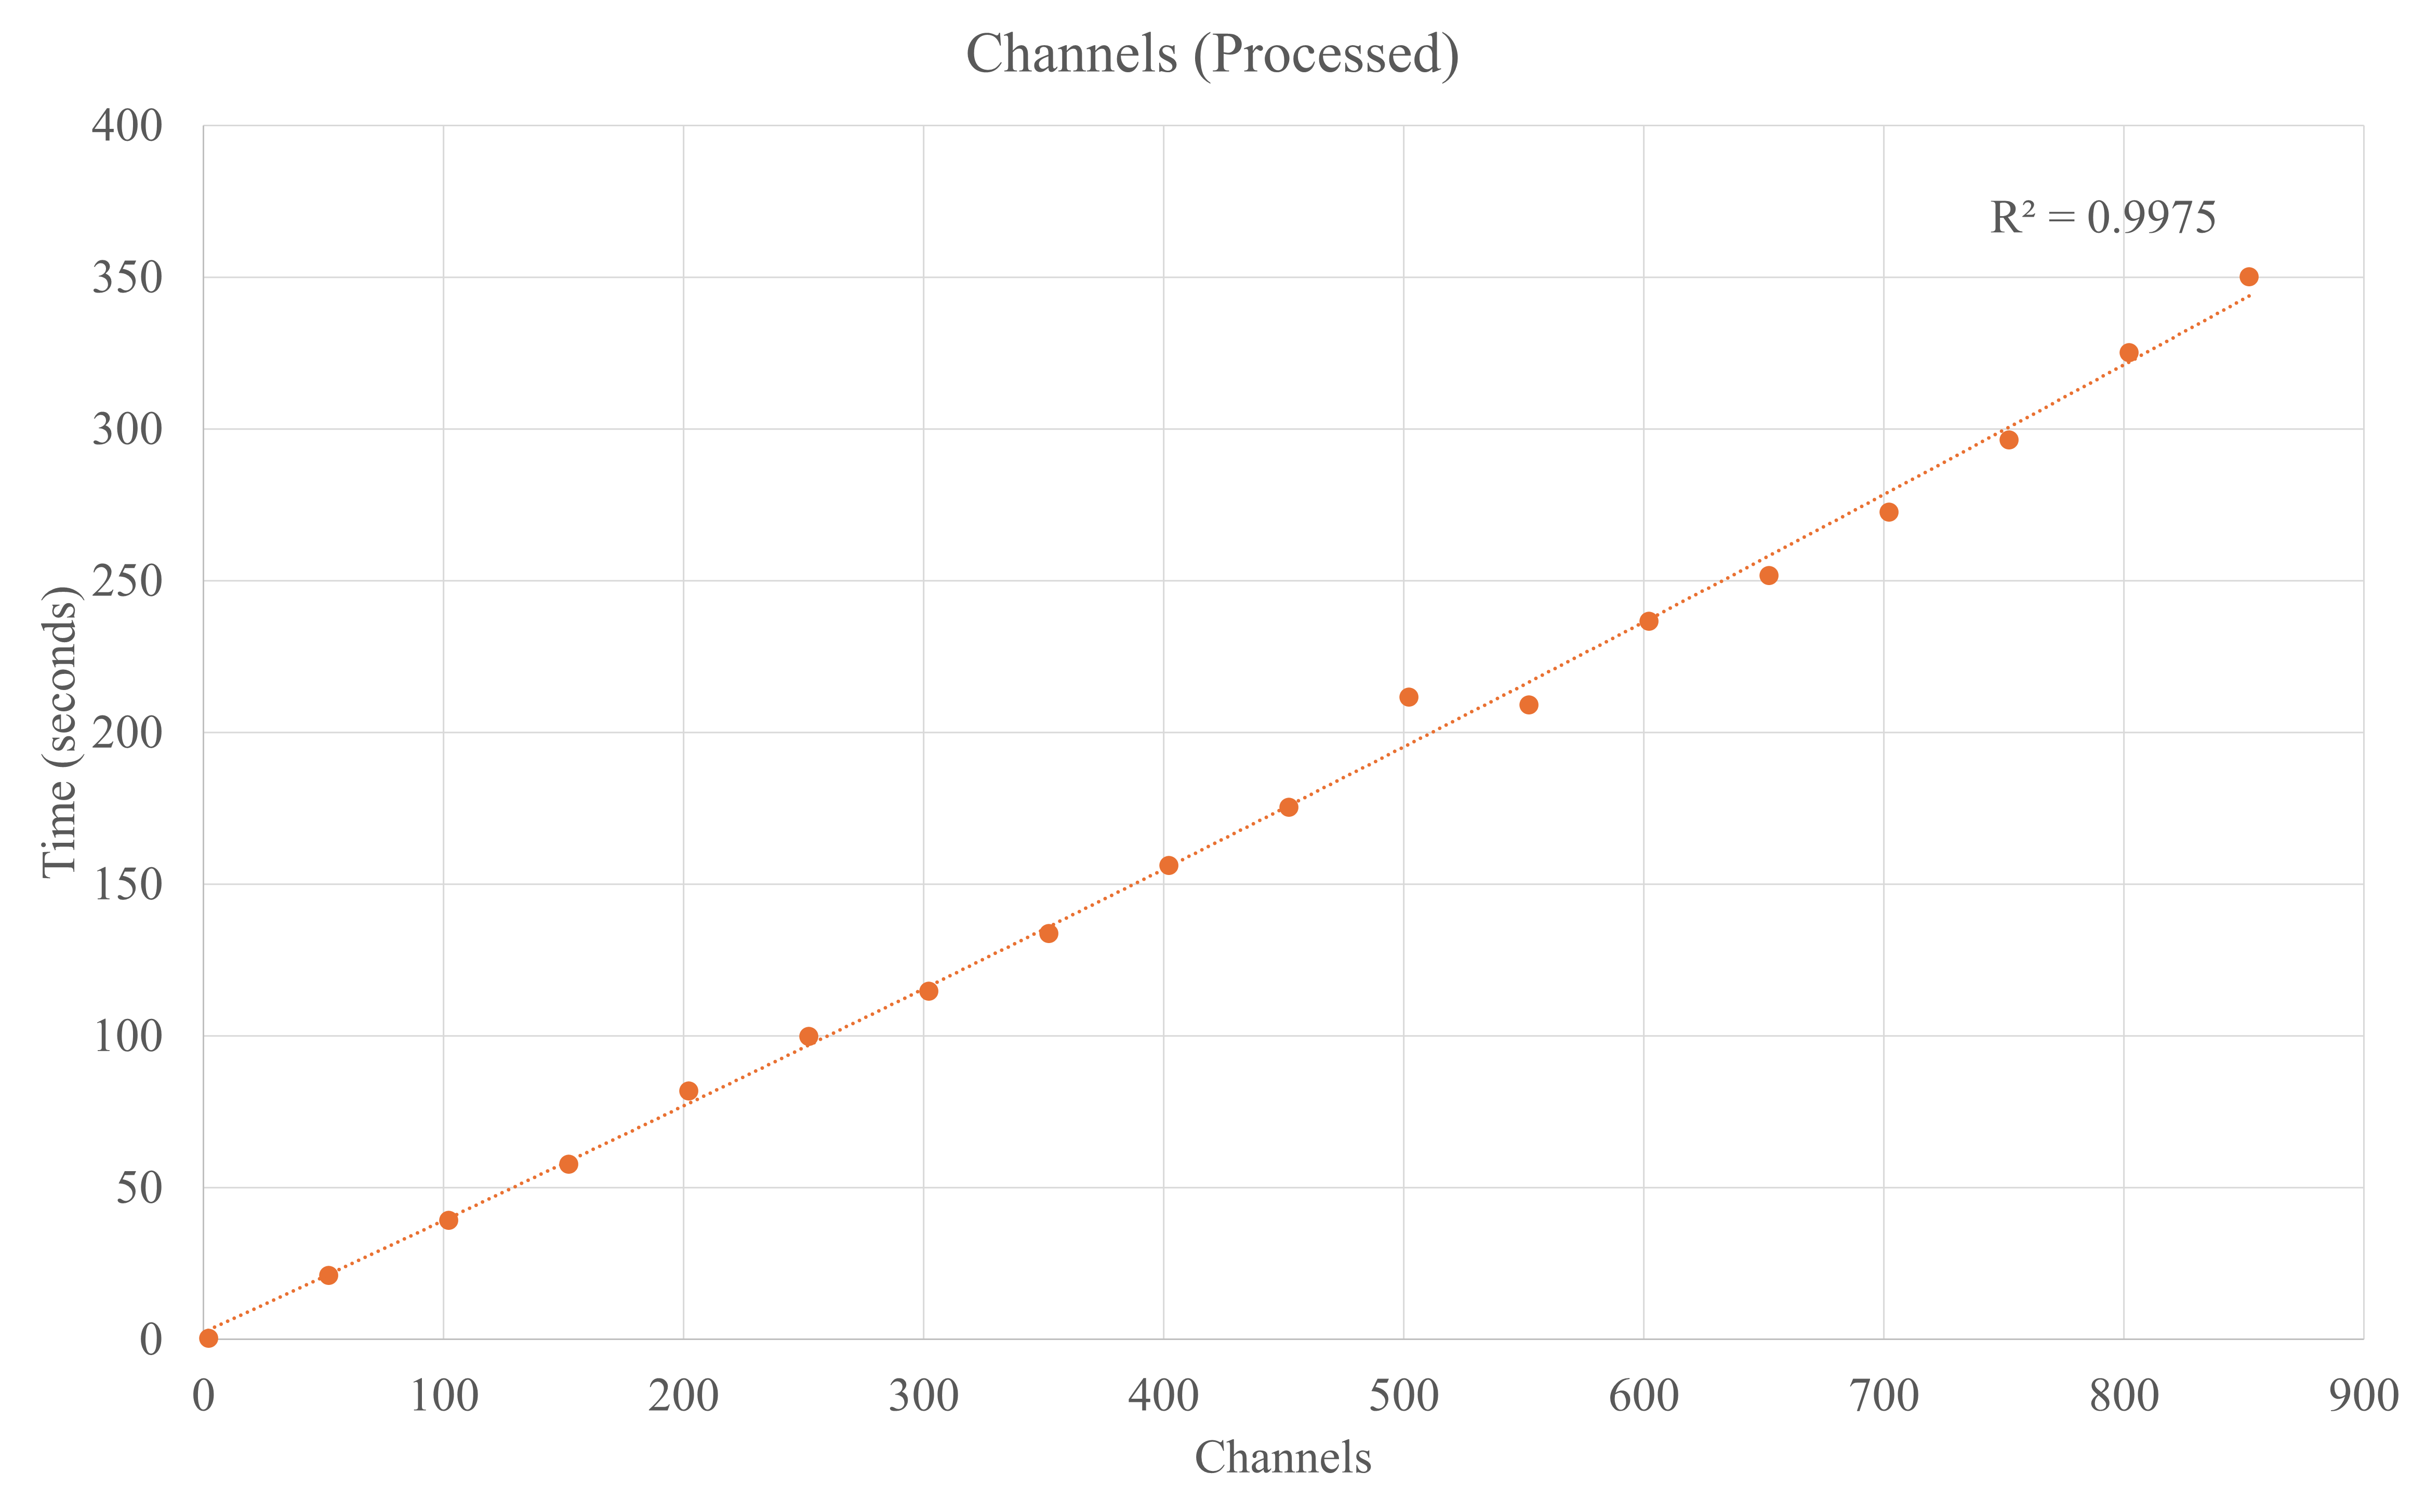
\includegraphics[width=0.75\linewidth]{ChannelsUnedited.png}
    \caption{Runtime for increasing Channels}
    \label{fig:ChannelsResults}
\end{figure}
\vspace{1mm}
\begin{figure}[h!]
    \begin{tabular}{cc}
        \subfloat[Raw Frequencies]{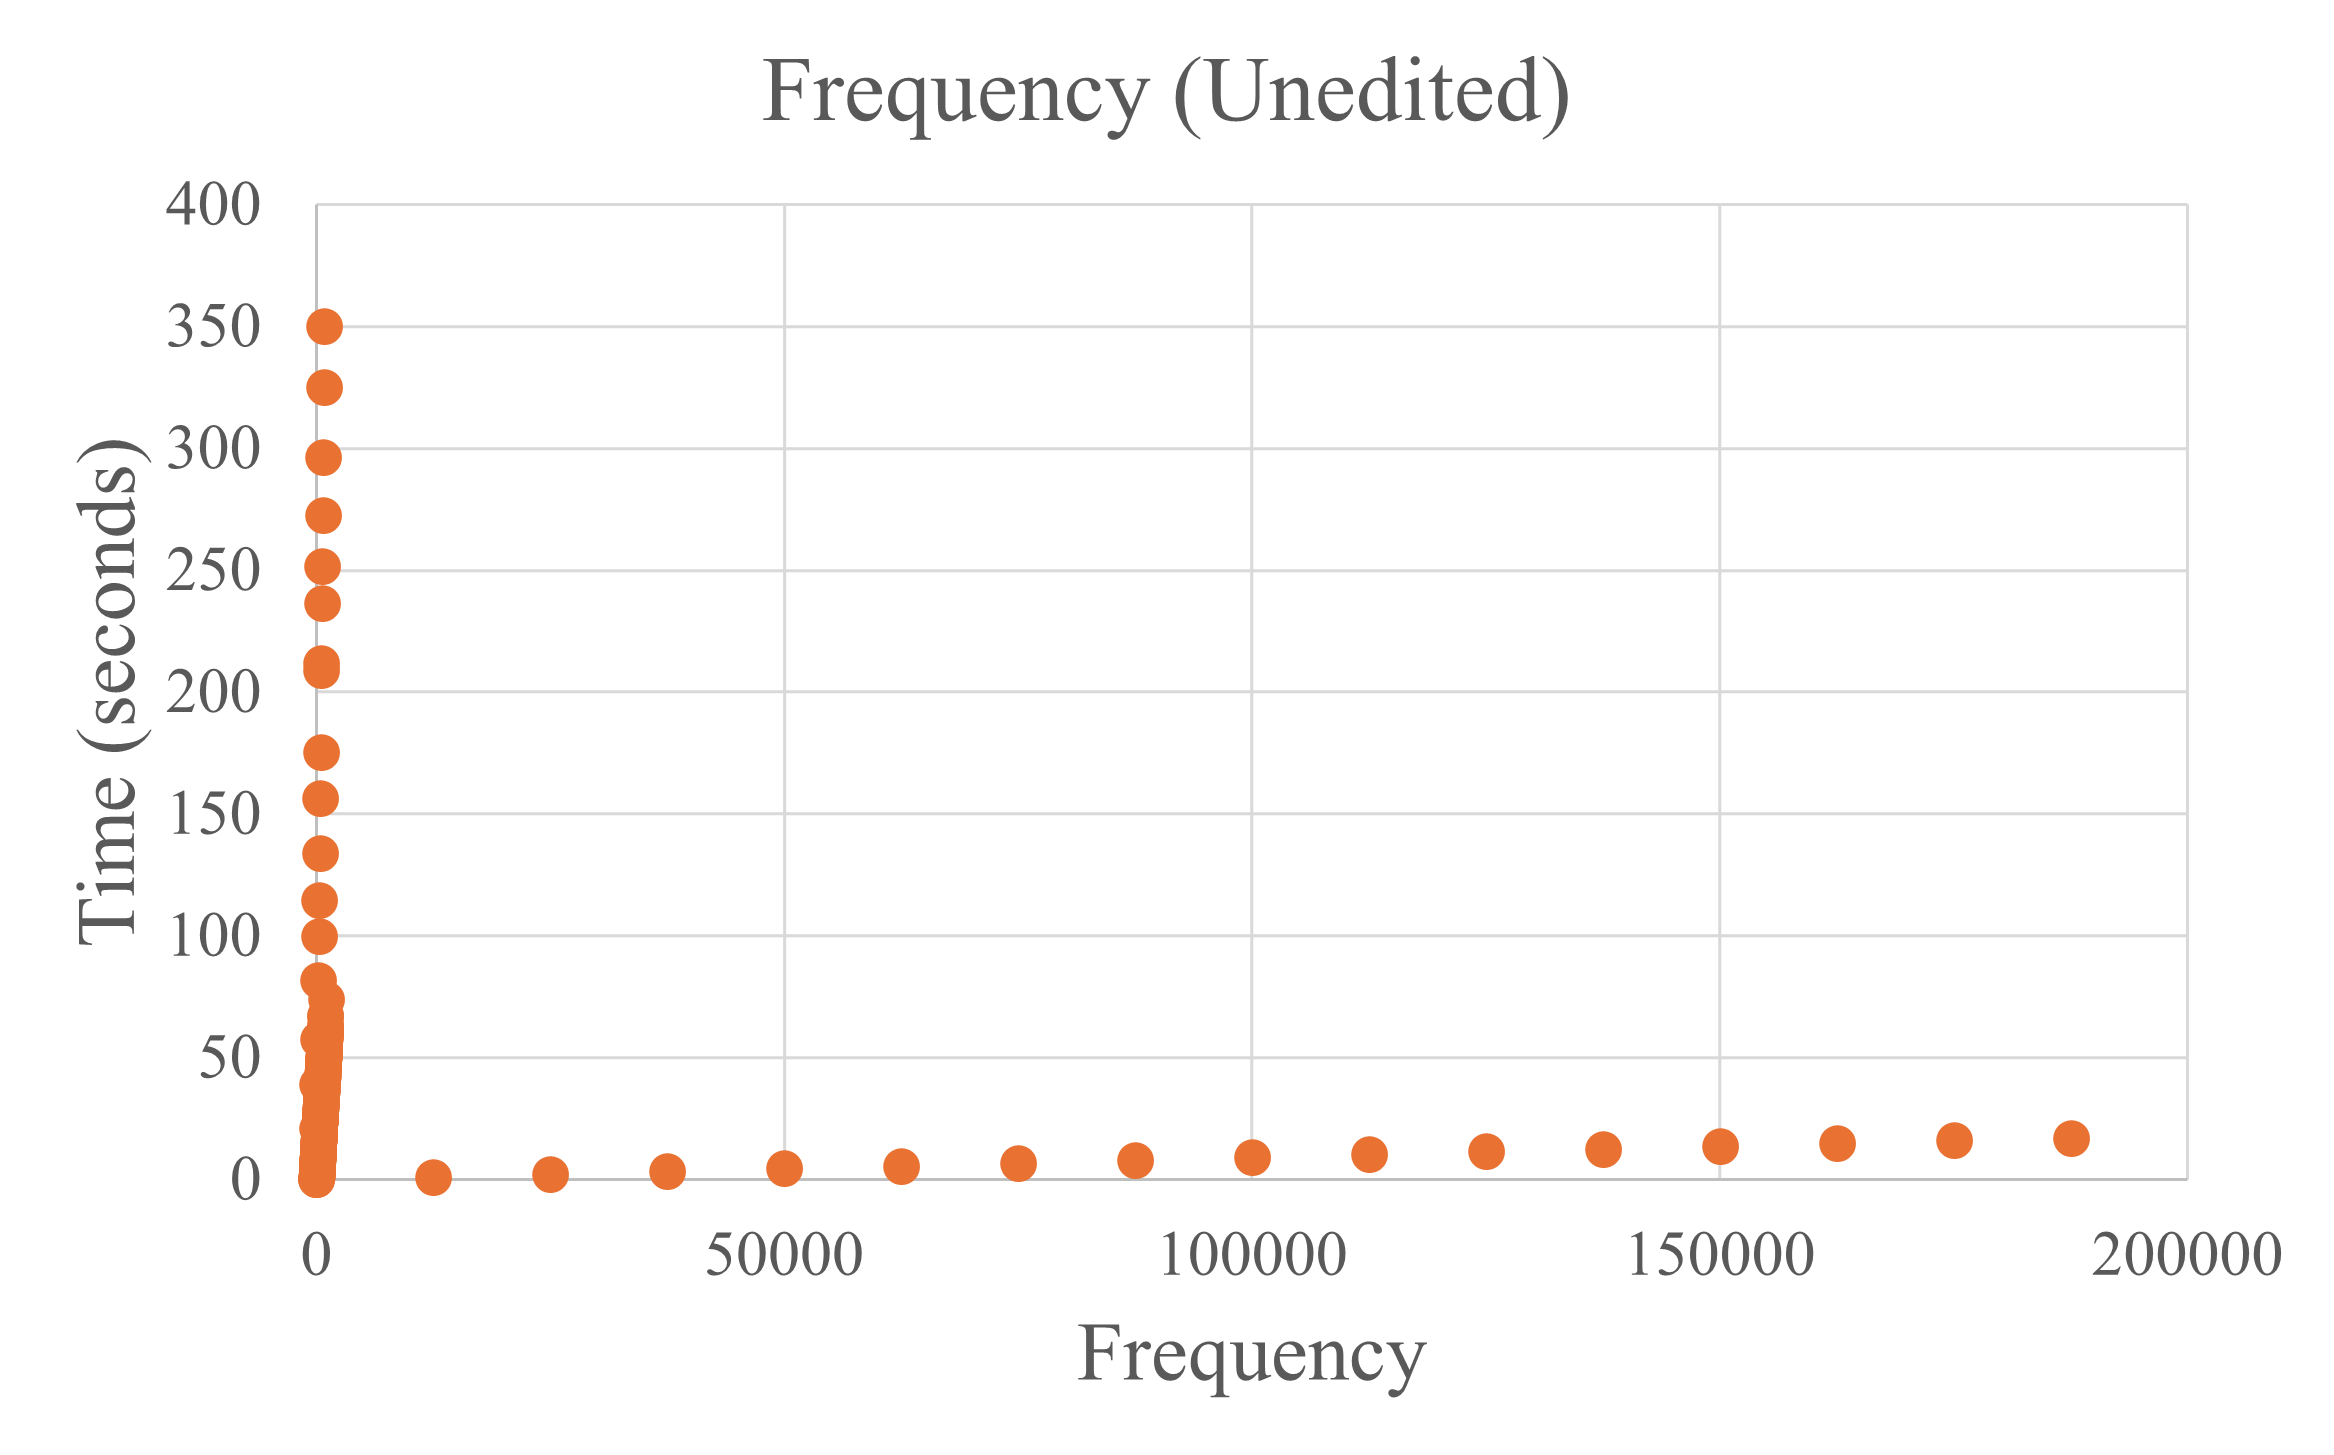
\includegraphics[width=0.45\linewidth]{FrequencyUnedited.png}}&
        \subfloat[Processed Frequencies]{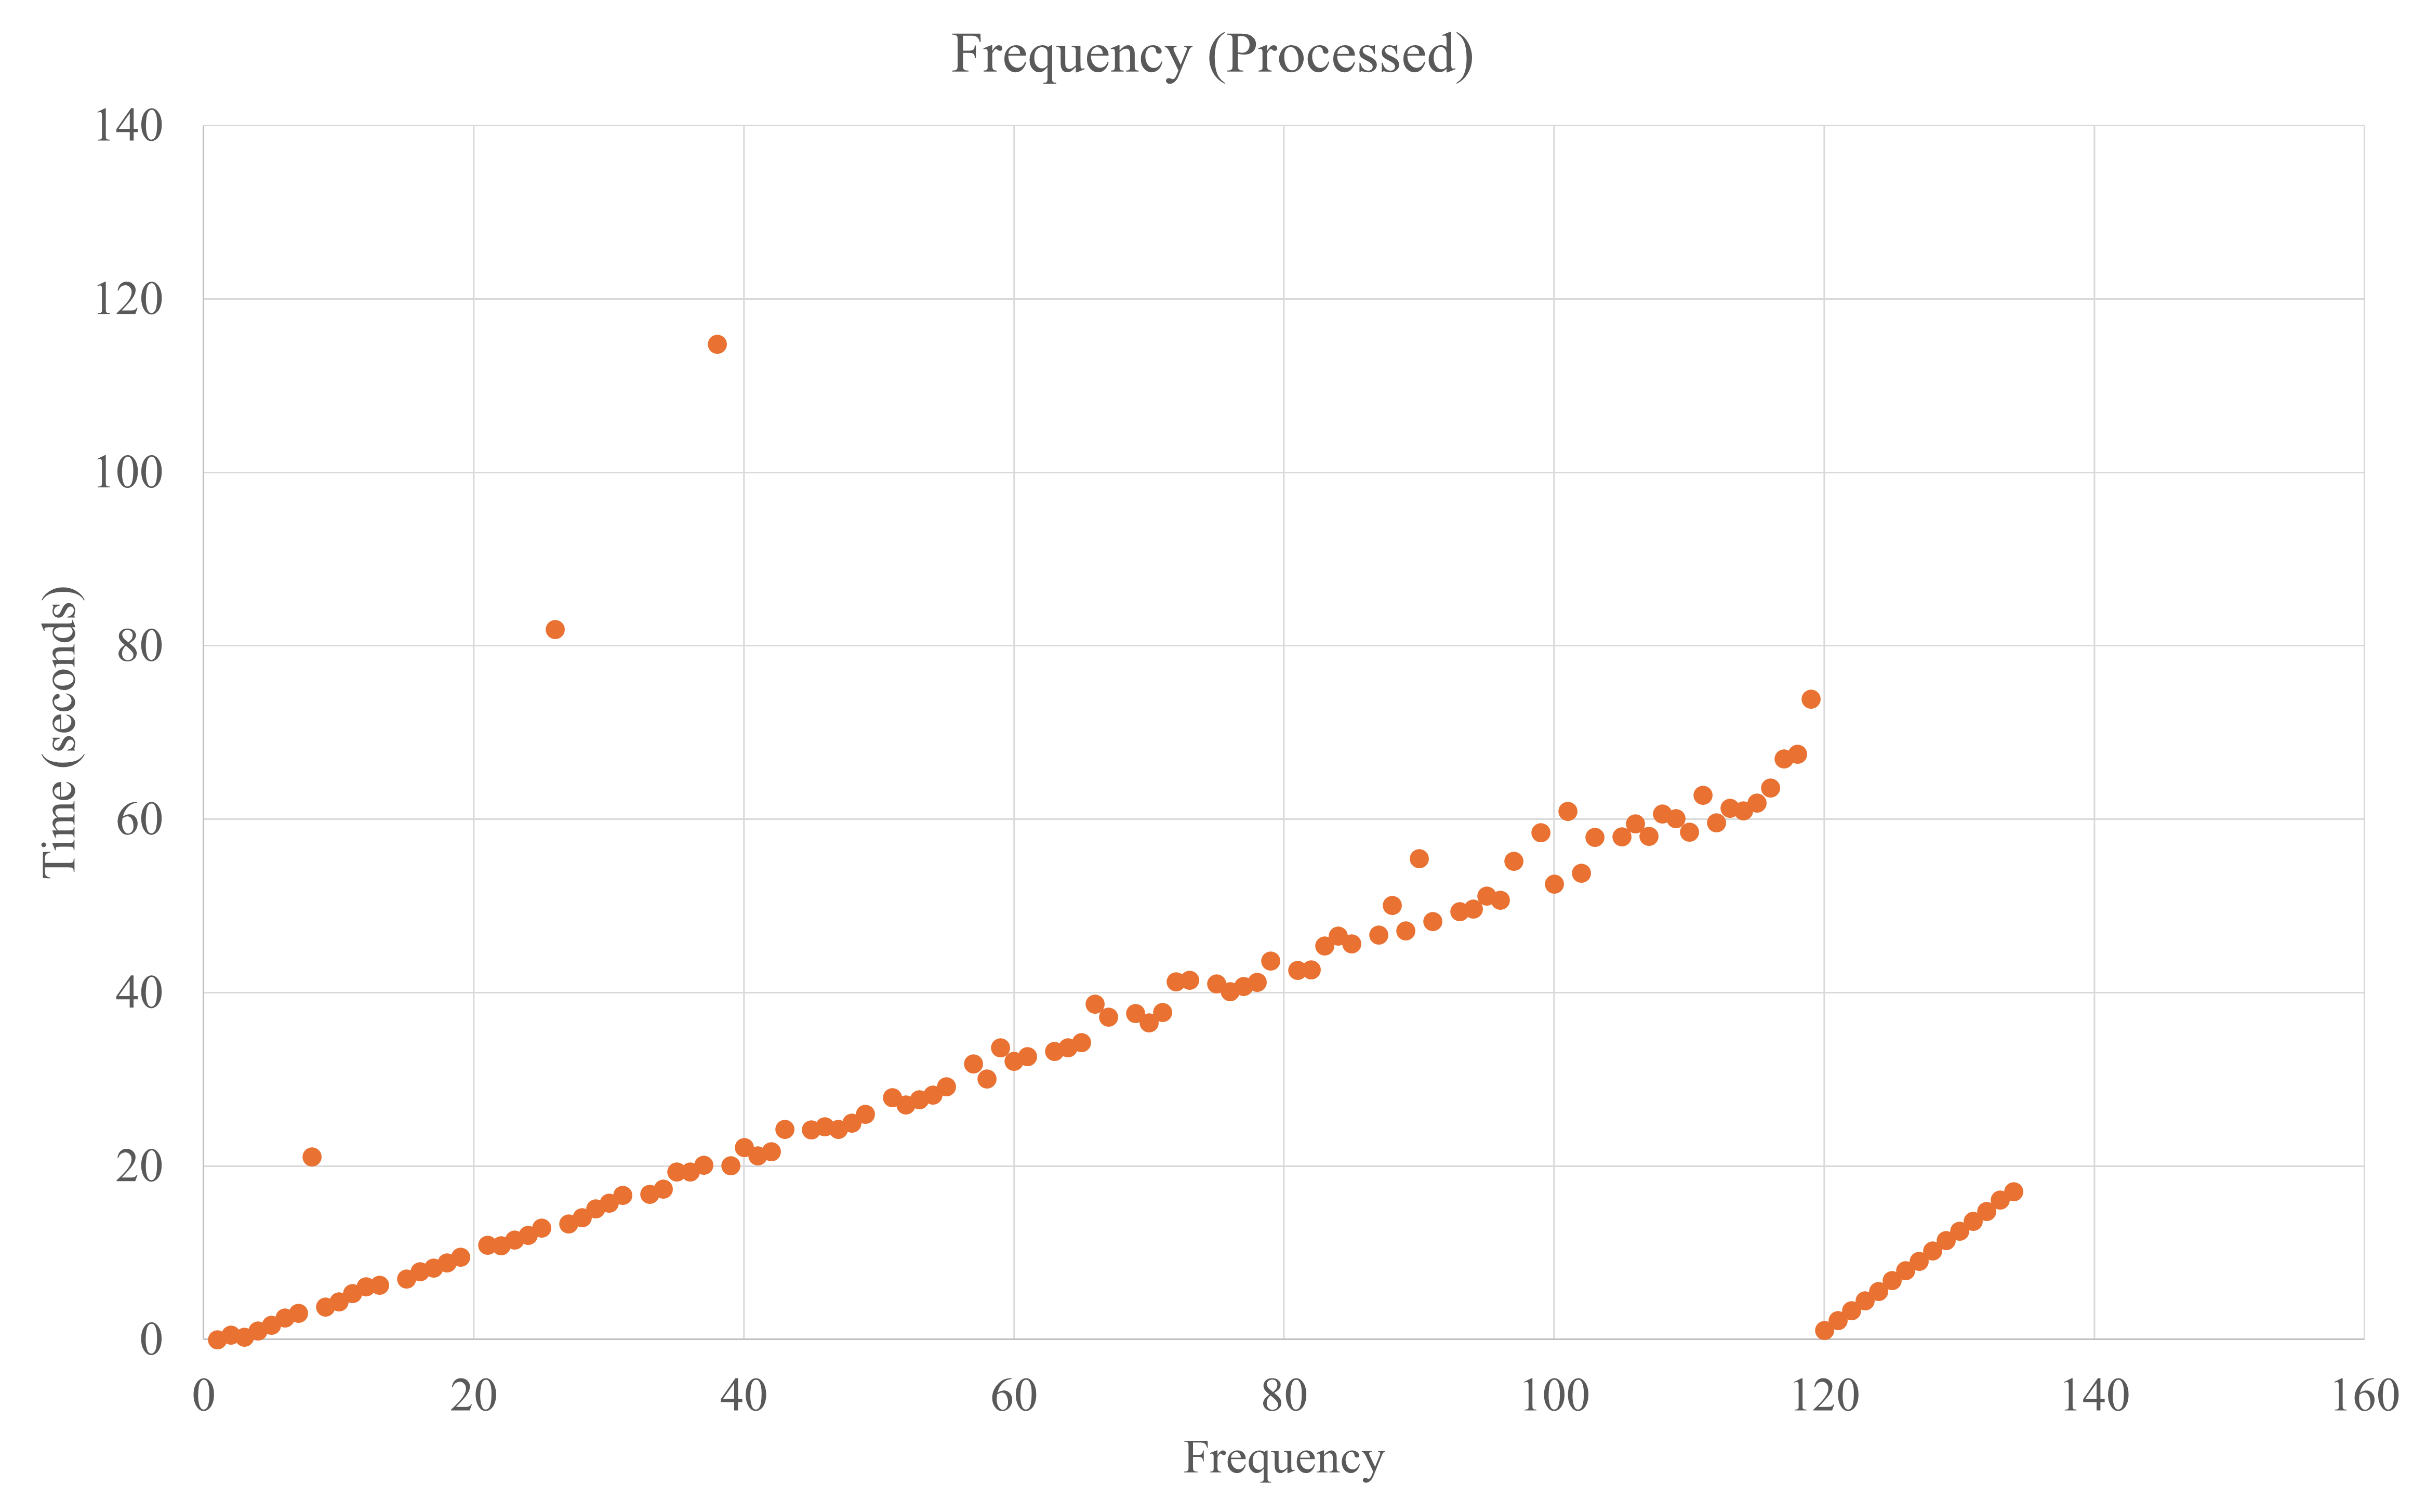
\includegraphics[width=0.45\linewidth]{FrequencyEdited.png}}
    \end{tabular}
    \caption{Runtime for increasing Frequency divisions}
    \label{fig:FrequenciesResults}
\end{figure}

Figures \ref{fig:PointsResults}, \ref{fig:ChannelsResults}, \ref{fig:FrequenciesResults} show the results
from BenchmarkTools. The reason for the two types of graphs was to remove outliers that skewed the data and prohibited
any analysis. Running the benchmark used all the free RAM available on my laptop as well as significant amounts of swap
space on my drive due to large amounts of overhead introduced by the BenchmarkTools benchmark. I believe that the
latency caused by IO to the swap file was the cause for the outliers and so I removed them in the edited graphs since
these points are not indicative of the actual performance of the library. After these points were removed, a curve was
fitted to each graph to provide an indication of the time complexity. From this analysis, I concluded that the runtime
of the library scales linearly ($\mathcal{O}(n)$) with the number of points, and quadratically ($\mathcal{O}(n^2)$) with
the number of channels. This aligns with expectations based on the code analysis of the DAS implementation. The main
beamformer loop consists of a single for loop iterating over the points as such, the algorithm is expected to behave
linearly with an increase in points. With channels, every additional antenna corresponds to a quadratic increase in
channels since every antenna can send to and receive from any other antenna in a fully multistatic system. This is
evidenced by the slight quadratic increase in Figure \ref{fig:ChannelsResults}. The algorithm is expected to have
$\mathcal{O}(n)$ growth since the frequency is only used once in the algorithm process to delay each signal, which is
evidenced by the linear growth in \ref{fig:FrequenciesResults}. Effectively, MERIT works very well with a large number
of points and with relatively few channels. This in turn affected the layout of the matrices in the library. Since data
to do with points would be accessed most frequently, the decision was made to place these along the columns of the
matrices. Since Julia is a column major language, this would provide the quickest access to this data. Data that relate
to the channels were placed along the second dimension since this would be accessed less frequently than data related to
the points. Finally, data relating to the frequency were placed along the third dimension, since this data is accessed
very infrequently, it was decided that the latency required to load this data from memory would be acceptable provided
it allowed us easy access to data relating to points and channels. The above graphs demonstrate the performance of the
MERIT.jl library. From limited testing on my laptop with an Intel i7-1185G7 CPU and 16GB of RAM, the Julia library
executed in the same amount of time as its MATLAB counterpart. However, further testing to accurately quantify the
runtime of both libraries is needed.

\section{MERIT.jl as a Library}
%%Talk about MERIT.jl as a library and talk about how its general. Compare and contrast with Tyson Rheimers python code.
\setcounter{chapter}{5}
\setcounter{section}{0}
\setcounter{subsection}{0}
\chapter*{Future Work}
\addcontentsline{toc}{chapter}{Future Work}
MERIT.jl in its current state already provides researchers with the tools to analyze and visualize scans and through the
integration of the aforementioned programming features, it achieves flexibility and extensibility. This chapter will
consider the scope of future work and how it can be integrated with MERIT.jl

\section{Time Domain Implementation}
\label{TDImplementation}
While this library focused on the frequency domain implementations of the beamformers, equivalent time domain
representations do exist, the main difference being the method in which the signals are delayed. One could extend the \lstinline[language=Julia]{delay_signal!} function in the Process.jl file to
accept signals that are subtyped from the Real abstract type. This way when working with time domain signals, the Julia
compiler, based on the principals of multiple dispatch, will select the correct implementation of the
\lstinline[language=Julia]{delay_signal!} function in a way that is fully transparent to the user. One could also extend
the \lstinline[language=Julia]{get_delay} function in Beamform.jl to accept a sampling rate as well as $\varepsilon$,
using the concept of closure, these variables would be captured and could be used to return the delay in terms of
samples instead of seconds. The functional implementations of the beamformers can stay as they are, as they sum over the
already delayed signals, they are indifferent to the numerical type of the input. 

\section{Implementation of More Beamformers}
The implementation of further beamformers can be an area for future work. Section \ref{JuliaScientificComputing} showed
how the structures and functions from multiple libraries could be combined behind the scenes to provide a more
streamlined experience for the end user. A similar idea could be implemented in MERIT.jl where the beamformers could be
defined in another library that gets used in MERIT.jl. The main benefit of this approach is that users are given the
option to download a ``lightweight'' version of the library with one beamformer if the particular choice of beamformer
does not matter, or they could install the secondary module and have access to a larger suite of beamformers. Another
benefit is that the developers of MERIT.jl need not concern themselves with having to implement all current and future
beamformers. This can be handled by a separate team thereby dividing the workload. Provided this team follows the
template of the DAS beamformer, they can have the guarantee that their function will also work in MERIT.jl.

\section{Parallel Processing}
Parallel processing was not a feature that was explored as it was outside the scope of this thesis. However, there are
areas of the code that have been identified as ``embarrassingly parallel''. These are sections of code that are amenable
to significant acceleration through the use of multithreading and parallel processing. Consider the beamforming equation
in equations \ref{eq:DASBeamformer, eq:DMASBeamformer}. For all of these, the response at each point is calculated
independently of the other points. As such this operation can be easily split across all available threads or even
all available GPU cores, providing exponential increases to the performance of the library overall. The Julia language
provides native support for threaded for-loops through the use of the \lstinline[language=Julia]{Threads.@threads}
macro, which will evenly split the for-loop range across the threads available to the Julia runtime. However, the onus
still lies on the user to ensure that no data race conditions can occur. Julia also supports GPU programming natively
through the use of CUDA.jl for Nvidia GPUs, AMDGPU.jl for AMD GPUs, oneAPI.jl for Intel GPUs as well as Metal.jl for the
current Apple integrated GPUs \cite{JuliaGPU}. However, one drawback to parallel processing is the increased logic
required to collect all the answers at the end. To prevent race conditions when writing to the output array, each
spawned thread would either have to acquire a lock on the final array in order to write to it or pass its calculated
answer to another thread that would sequentially write to the output array. In both cases, the performance provided by
parallelizing the code would be hampered by the overhead introduced by collecting the results. 
\setcounter{chapter}{5}
\setcounter{section}{0}
\setcounter{subsection}{0}
\chapter*{Conclusions}
MERIT.jl was created to answer the question, "
% note that your supervisor may have a strong opinion on the style of referencing you use. Some background is available at https://www.overleaf.com/learn/latex/Bibtex_bibliography_styles
\bibliographystyle{IEEEtran} %Changed to IEEETran by HS
%\bibliographystyle{unsrt}

\bibliography{citations.bib}
\appendix
\renewcommand{\thechapter}{A\arabic{chapter}}


\end{document}